% !TEX root = thesis.tex

\chapter{Summary}

Our world is three-dimensional and complex, continuously changing over time and appearing different at different scales.
Yet, when we model it in a computer using Geographic Information Systems (GIS), we mostly use 2D representations, which essentially consist of linked points, lines and polygons (\reffig{fig:brep-sum-en}).
\marginpar{
\captionsetup{type=figure}
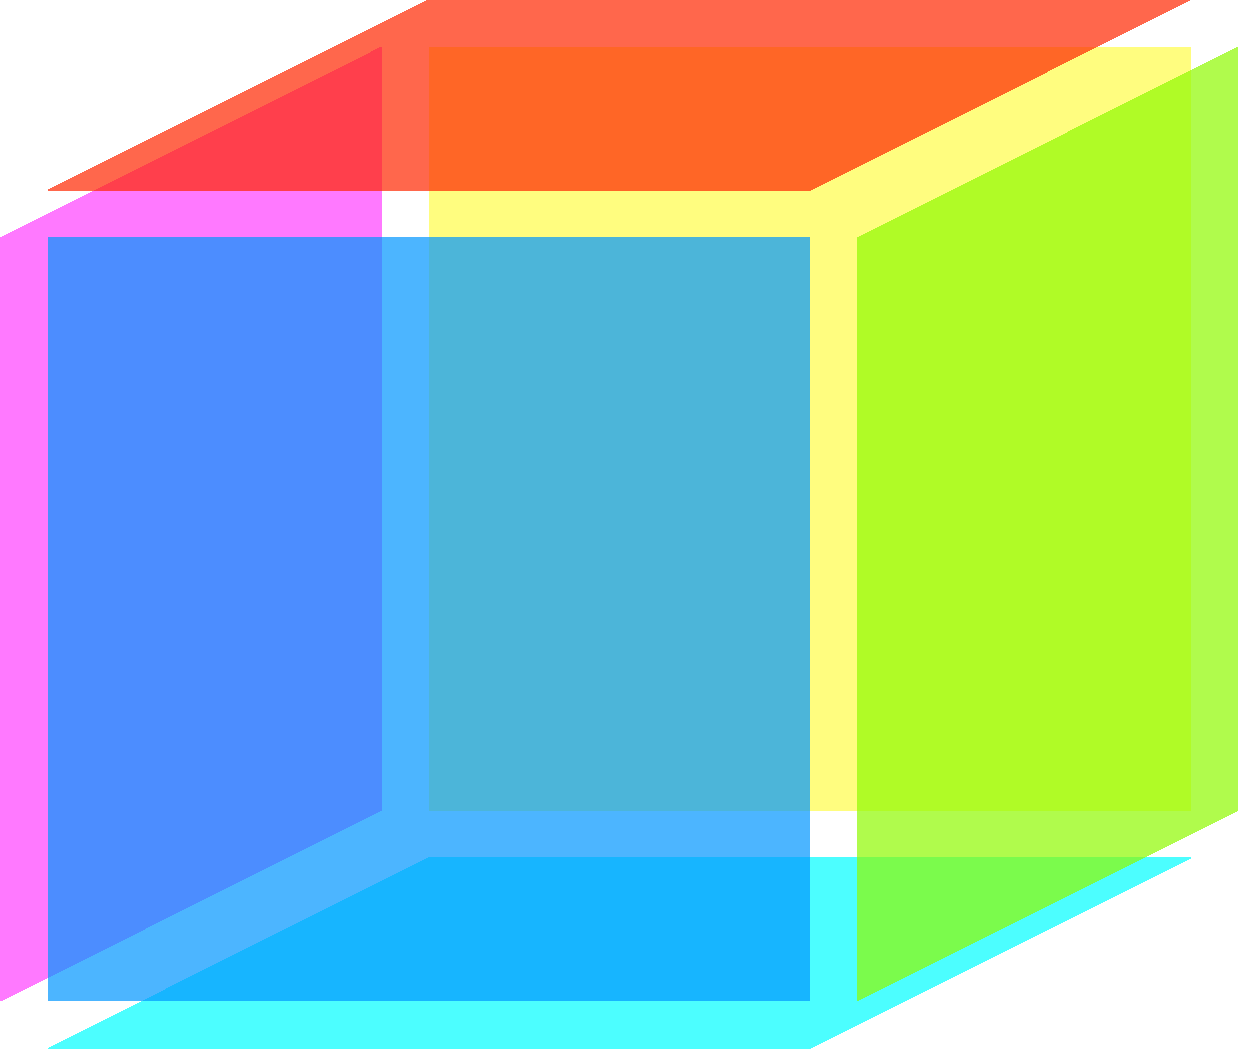
\includegraphics[width=\marginparwidth]{figs/brep}
\caption[A cube represented as the 6 square faces that bound it]{In GIS, a cube is not represented as a 3D solid, but as the 6 square 2D faces that bound it.}
\label{fig:brep-sum-en}
}
These representations are relatively easy to use and efficient, and a wide variety of methods is built on top of them.
However, 2D representations are necessarily limiting.
They force us to reduce problems to two dimensions, limit the type of objects we can represent, and complicate storing the relationships between different objects---especially when these are across time and different scales.
Nevertheless, most research in GIS is devoted to improving these 2D representations, as well as to the development of new methods that build on them to solve problems, both old and new.

This thesis explores a new, fundamentally different modelling approach---integrating both spatial and non-spatial characteristics as dimensions in the geometric sense, specifically targeting the cases of time and scale (\reffig{fig:axes-sum-en}).
\marginpar{
\captionsetup{type=figure}
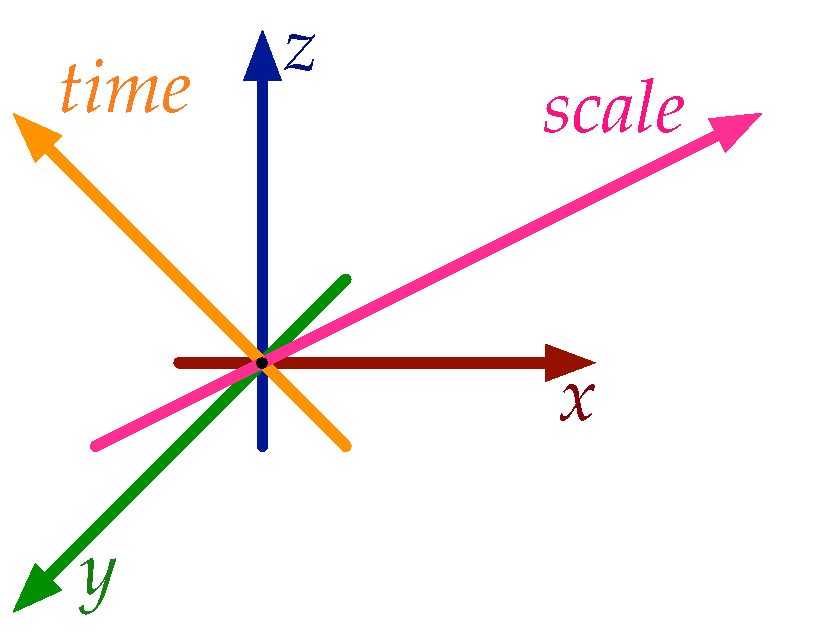
\includegraphics[width=\marginparwidth]{figs/axes}
\caption{3D space, time and scale can be modelled as 5D space.}
\label{fig:axes-sum-en}
}
While this has been proposed before at a conceptual level, this thesis aims to \emph{realise the fundamental aspects of a higher-dimensional GIS} by developing higher-dimensional ($n$D) representations, as well as new methods operating on them to create, manipulate and visualise geographic information.
As this thesis shows, the higher-dimensional approach is undoubtedly memory-intensive, but it is also very powerful, as it provides a simple and consistent way to store geometry, attributes and the topological relationships between objects of any dimension.
This generic approach can also be easily extended to handle other non-spatial characteristics, enabling better data management that is consistent across dimensions and more powerful operations, such as checking if two objects are adjacent at any point in time.

In order to model higher-dimensional space, it is best to consider an $n$D space subdivision as a base (\reffig{fig:space-filling-sum-en}), which is conceptualised as an $n$-dimensional simplicial complex or cell complex.
\marginpar{
\captionsetup{type=figure}
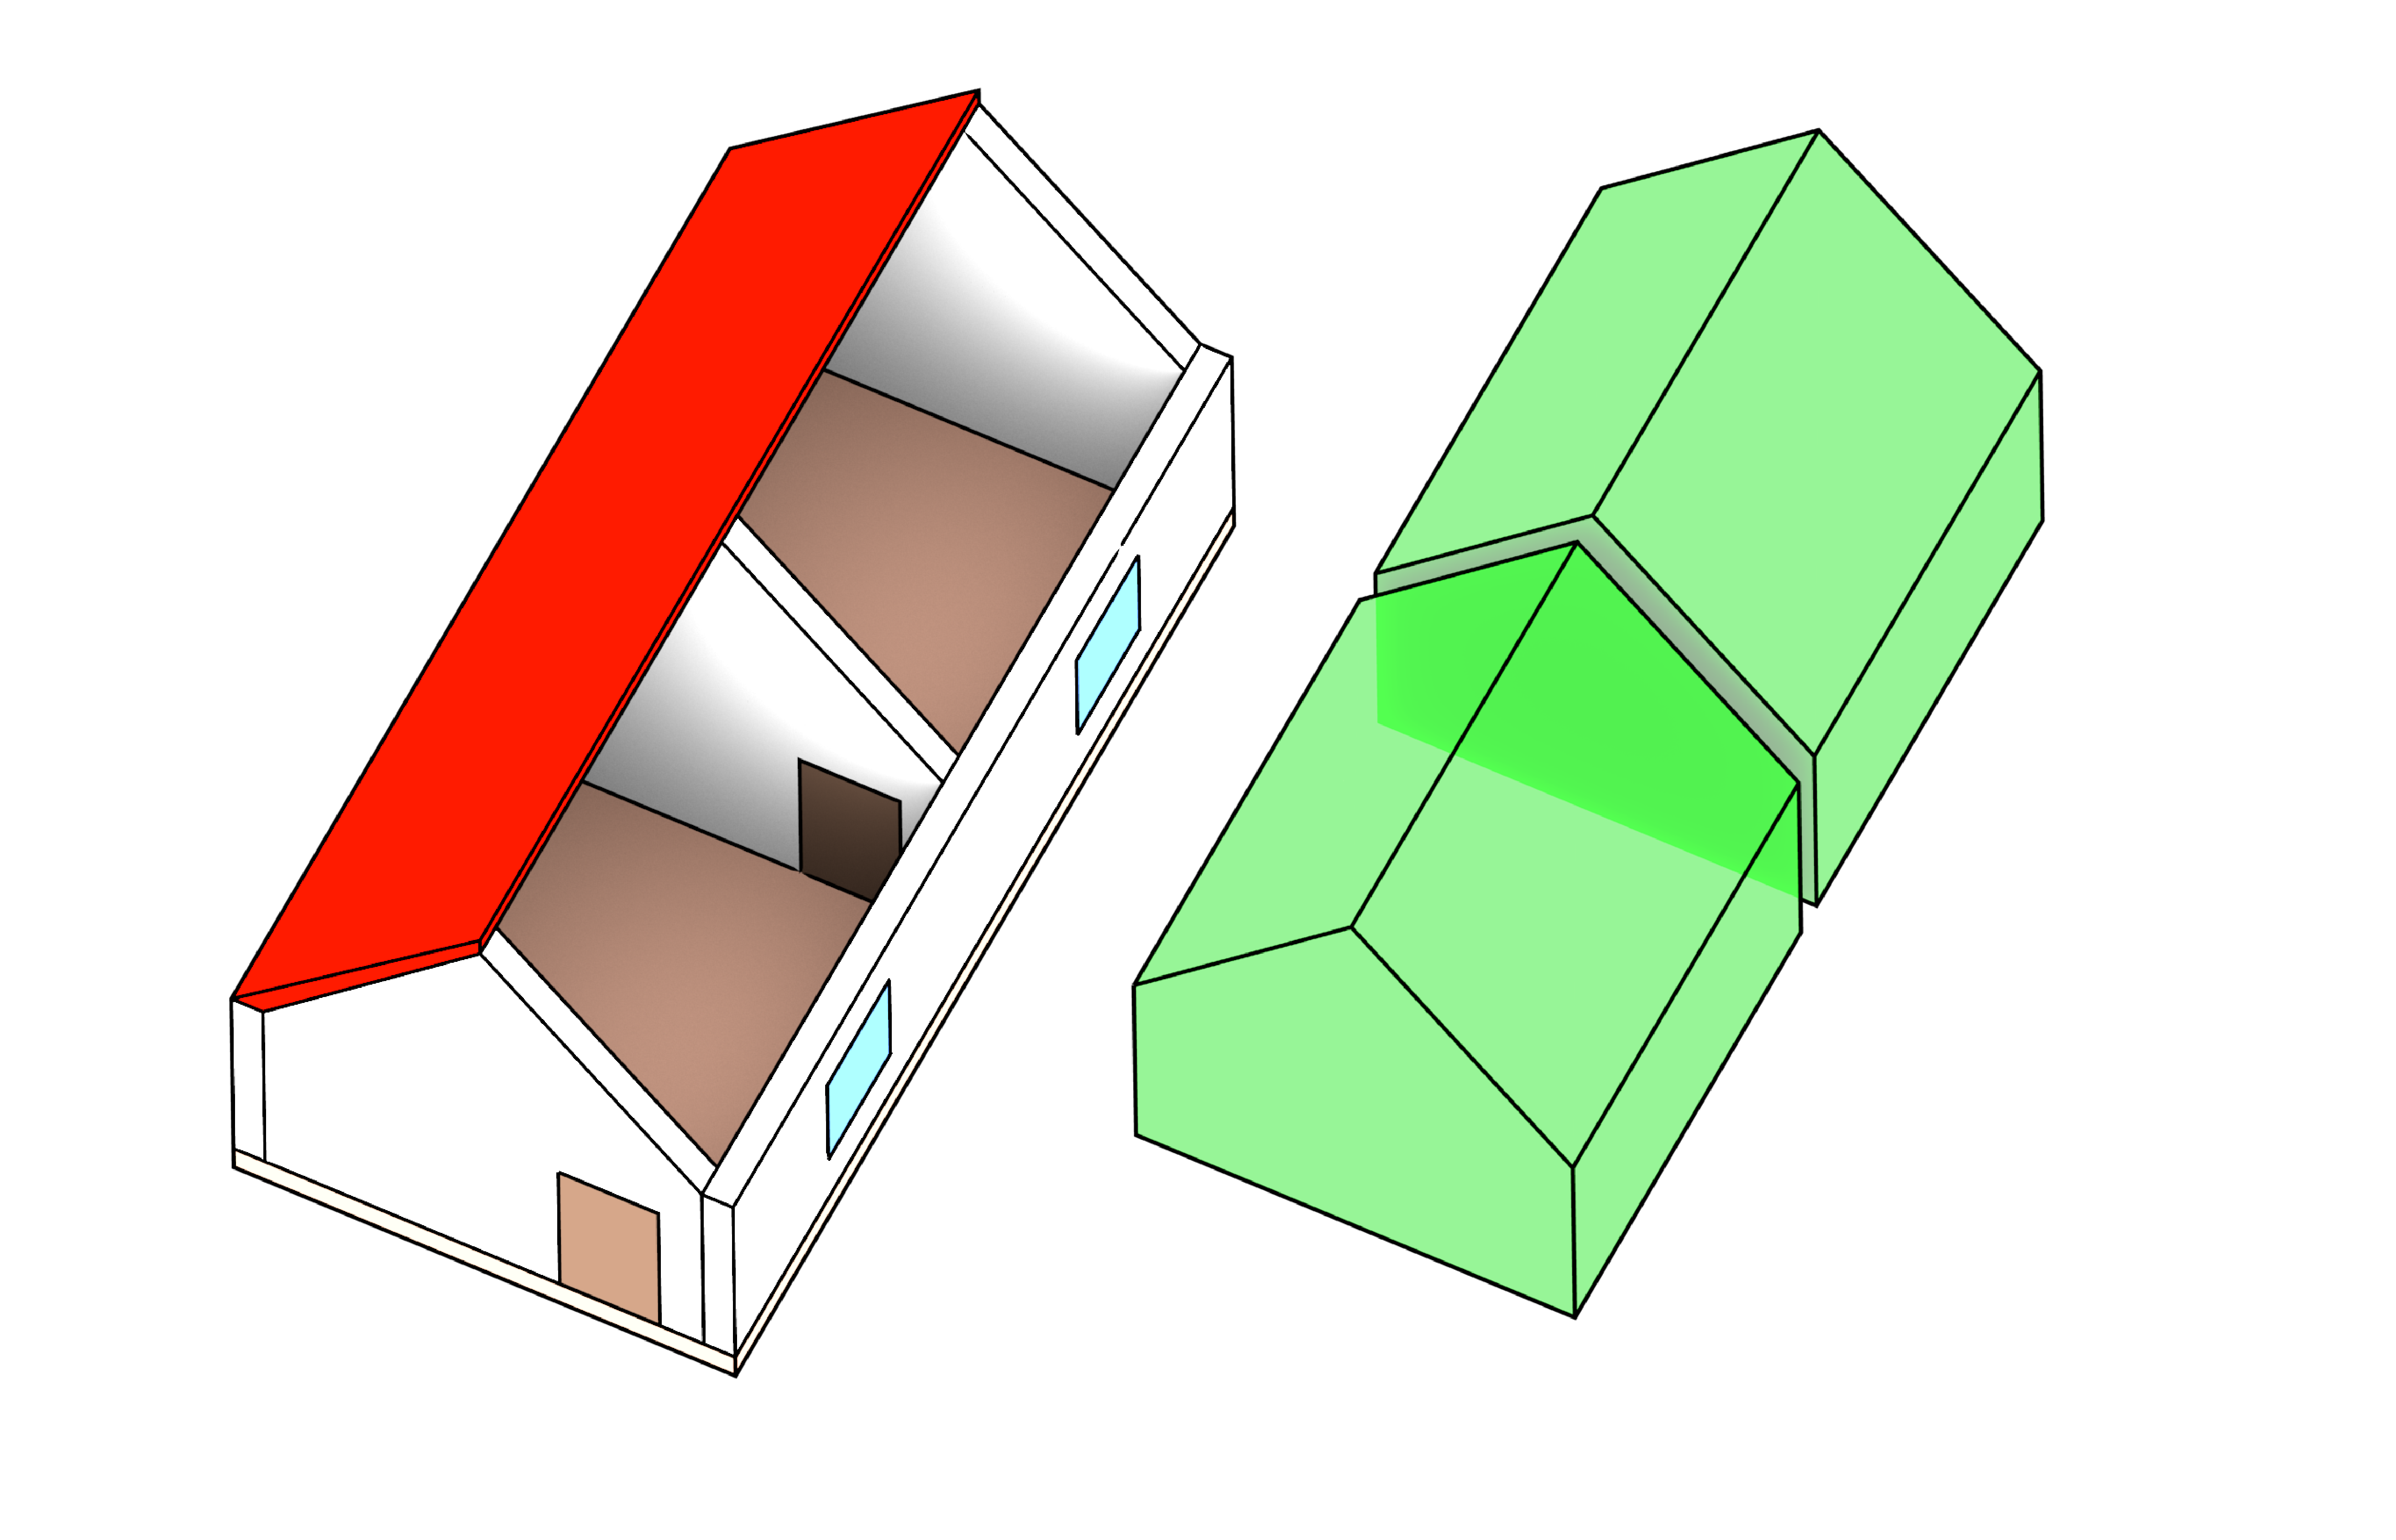
\includegraphics[width=\marginparwidth]{figs/space-filling}
\caption[3D space subdivision model]{A 3D space subdivision model is composed of a set of space-filling volumes without gaps or overlaps.}
\label{fig:space-filling-sum-en}
}
This can then be implemented with a simplex-based data structure, with an incidence graph, as a set of Nef polyhedra, or---as done in this thesis---by using ordered topological models such as the cell-tuple and generalised/combinatorial maps.

Creating computer representations of higher-dimensional objects can be complex.
\marginpar{
\captionsetup{type=figure}
\subfloat[]{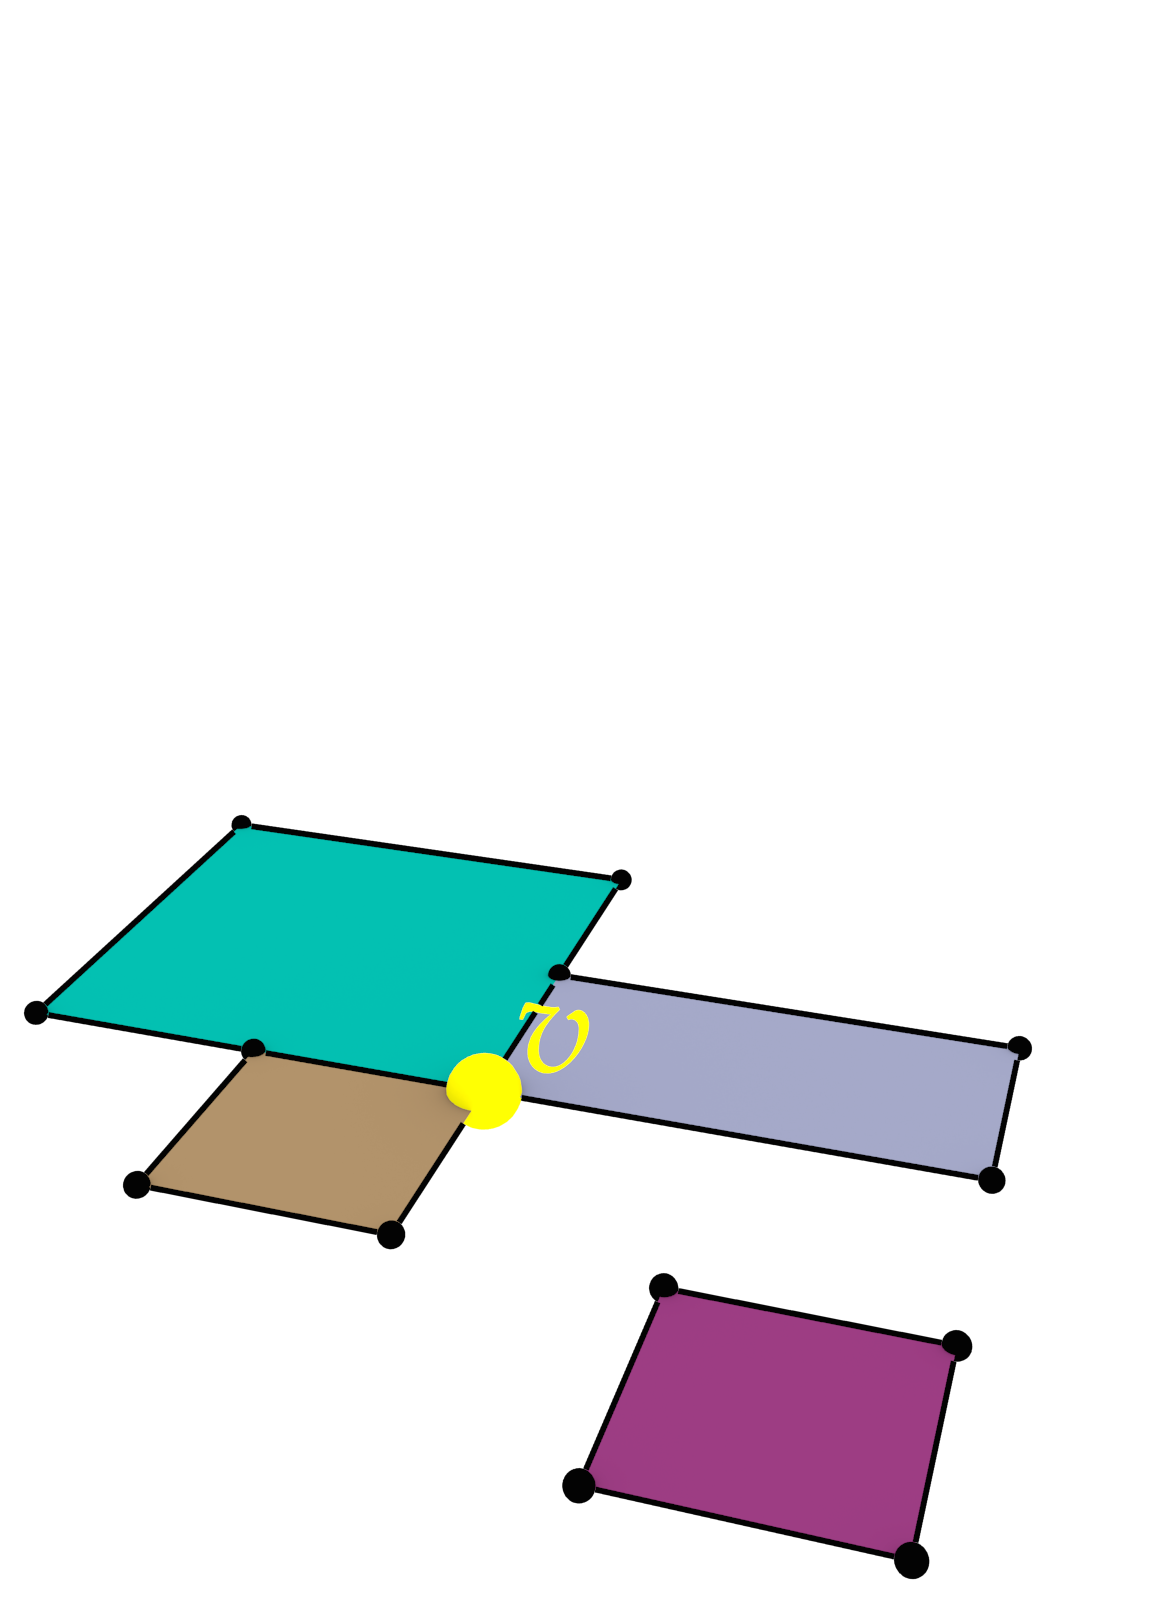
\includegraphics[width=\marginparwidth]{figs/extrusion-1}}\\
\subfloat[]{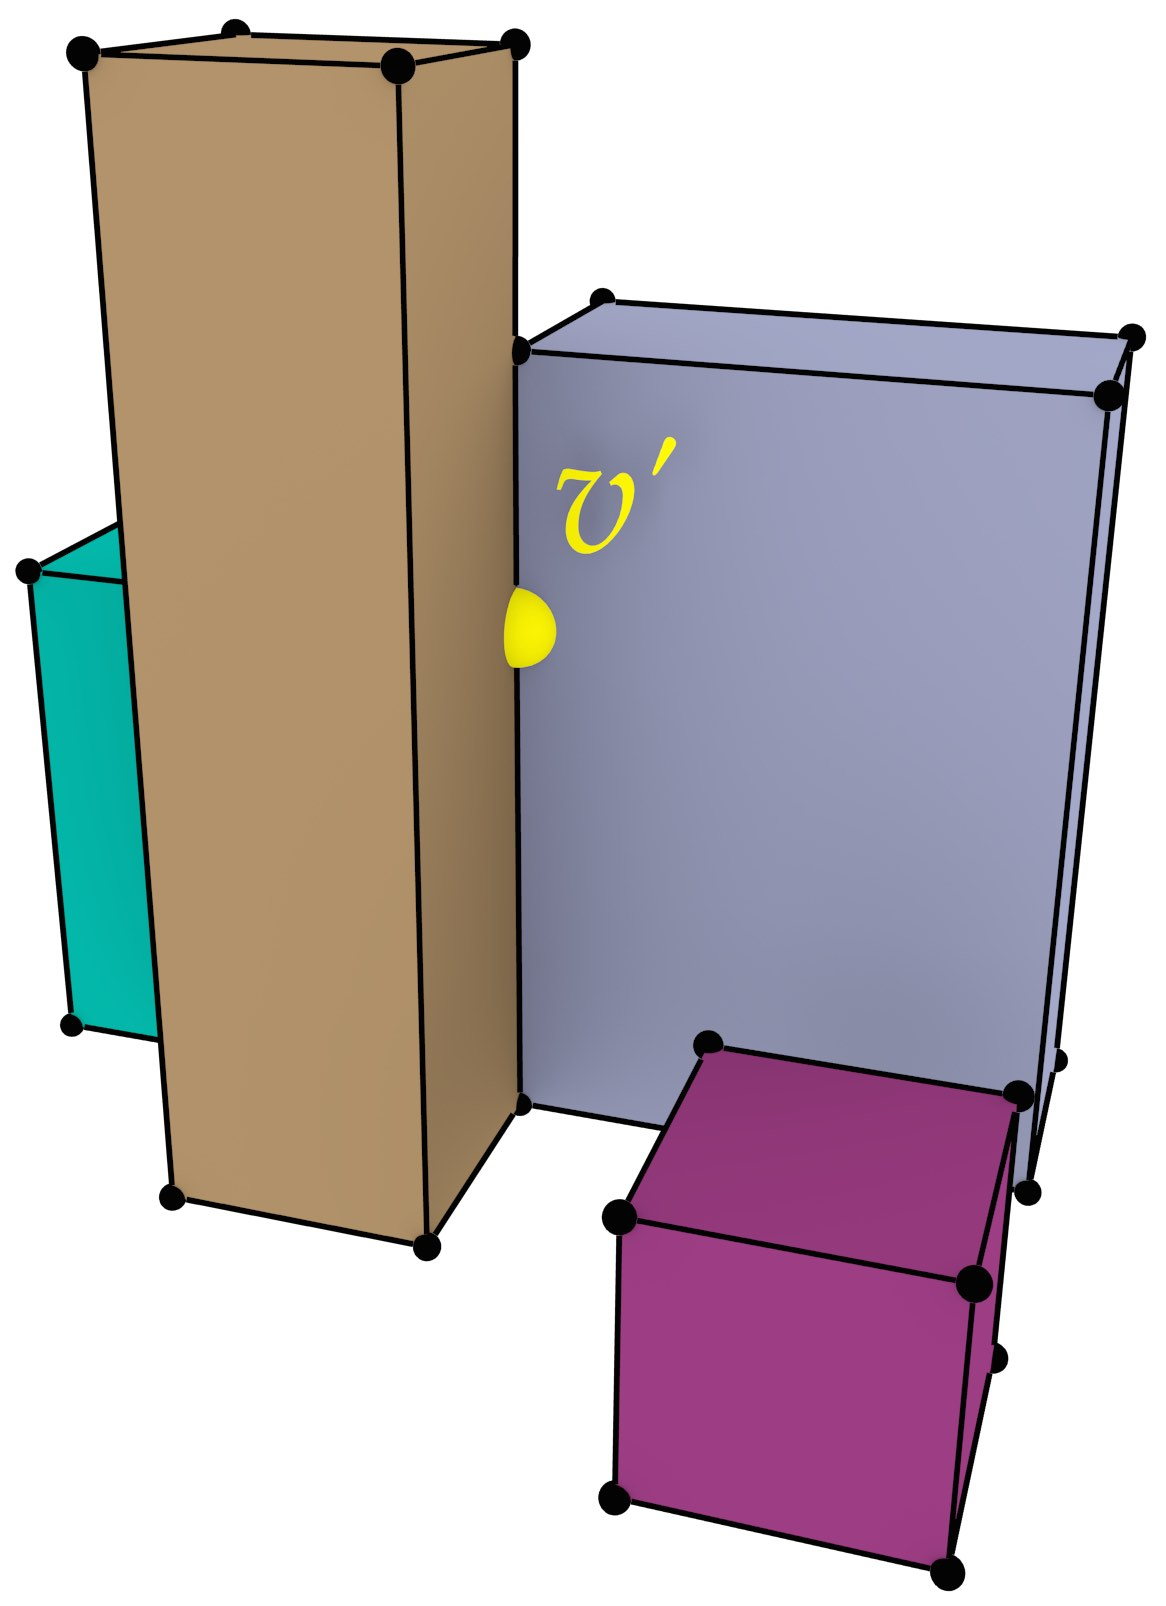
\includegraphics[width=\marginparwidth]{figs/extrusion-2}}
\caption[A set of polygons is converted into a set of boxes by 2D-to-3D extrusion.]{(a) A set of polygons is converted into (b) a set of boxes by 2D-to-3D extrusion.}
\label{fig:extrusion-sum-en}
}
\marginpar{
\captionsetup{type=figure}
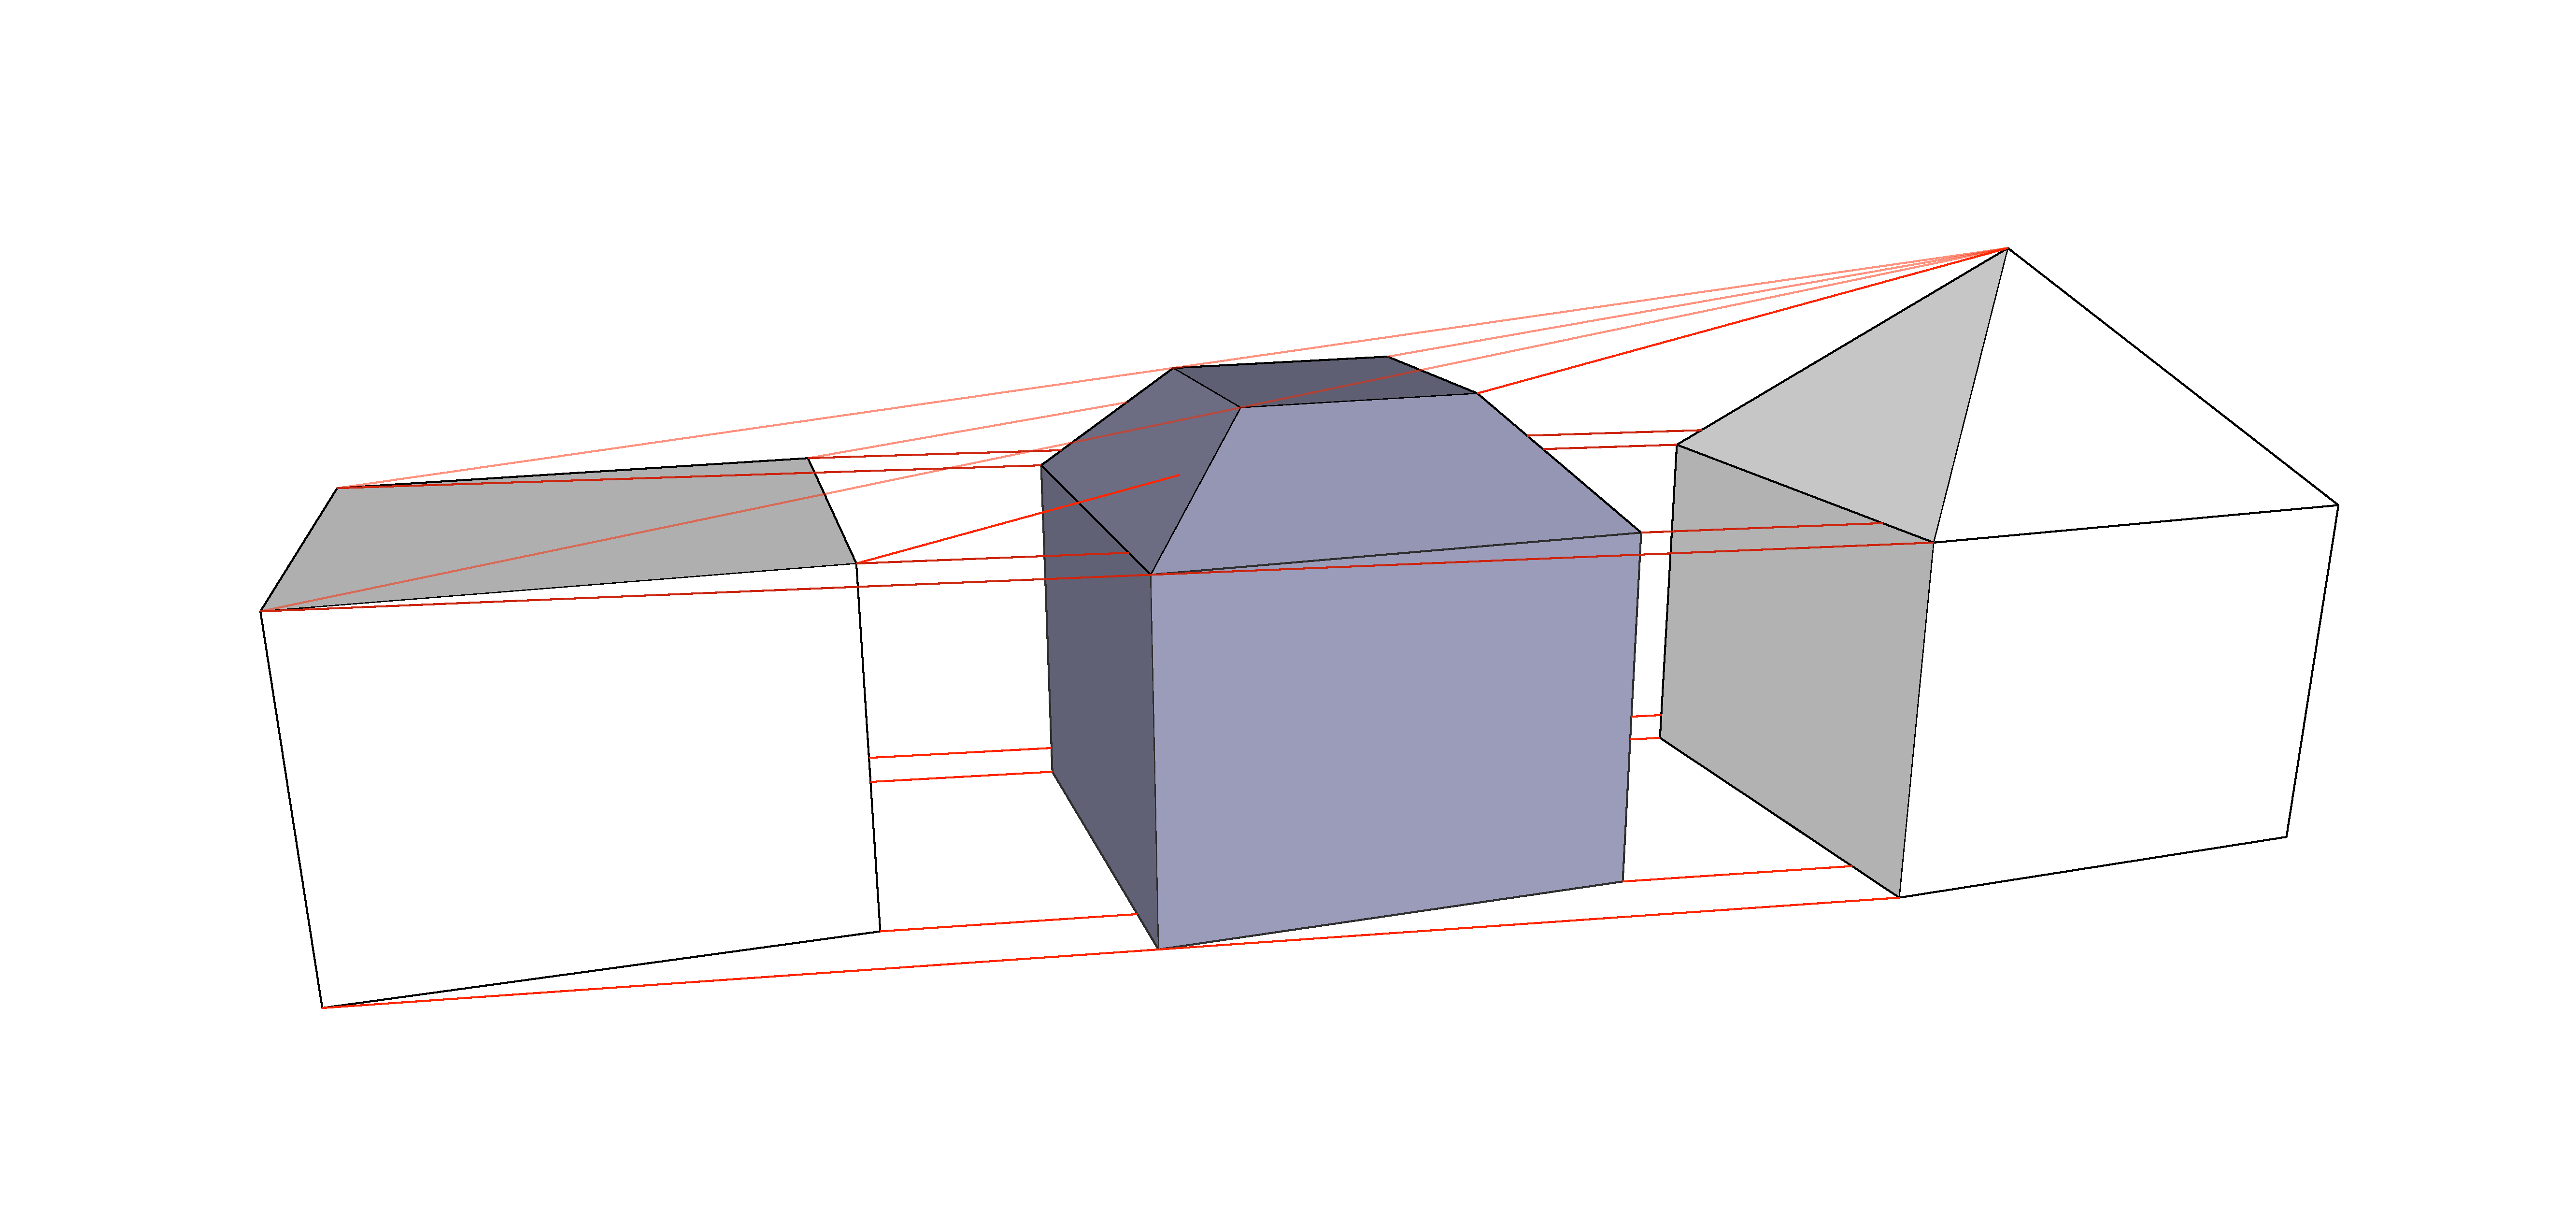
\includegraphics[width=\marginparwidth]{figs/link2}
\caption[Two LODs of a 3D model of a house are linked into a 4D model]{Two LODs of a 3D model of a house (left and right) are linked into a 4D model.}
\label{fig:link-sum-en}
}
Common construction methods used in 2D and 3D, such as directly manipulating combinatorial primitives, or using primitive-level construction operations (such as Euler operators), rely on our intuition of 2D/3D geometry, and thus do not work well in higher dimensions.
It is therefore all too easy to create invalid objects, which then cannot be easily interpreted or fixed---a problem that is already exceedingly apparent in three dimensions.

As a way to easily create representations of higher-dimensional objects, this thesis proposes three novel higher-level methods, all of which are intuitive to use and attempt to create valid output.
\emph{Extrusion} takes an $(n-1)$-dimensional cell complex and a set of intervals per cell, projecting them parallel to a new axis in order to create an $n$-dimensional cell complex (\reffig{fig:extrusion-sum-en}).
\emph{Incremental construction} describes an $n$-dimensional object based on its $(n-1)$-dimensional boundary, from dimension zero (points) and then upwards.
Finally, a 4D model can be constructed from a series of 3D models at different levels of detail (LODs) by \emph{linking them} (\reffig{fig:link-sum-en}).

In order to visualise higher-dimensional models, as well as to be able to process them in existing software, it is important to have methods to extract meaningful 2D/3D subsets from them.
% Such methods would consist of two steps: (i) selecting a subset of the objects in the model and (ii) projecting this subset to a lower dimension.
As a stepping stone towards such methods, this thesis shows how $n$-dimensional to ($n-1$)-dimensional orthographic and perspective projections can be defined.

Finally, this thesis placed an emphasis on validating the algorithms with real-world datasets, which was only possible by developing methods to repair the invalid datasets that are widespread in practice.
This thesis thus contains methods to create valid polygons and planar partitions using a constrained triangulation of the input, as well as a method to repair polyhedra and space subdivisions by snapping together lower-dimensional primitives and removing overlaps using Boolean set operations on Nef polyhedra.
This allowed tests with up to 6D datasets based on real-world data---\emph{a good base for higher-dimensional GIS}.

In the future, the work in this thesis will be extended with higher-dimensional modification operations, true 4D spatiotemporal datasets and repair methods with quality guarantees.
All implementations made for this thesis are publicly available under open source licences.

\chapter{Samenvatting (Dutch summary)}

{\selectlanguage{dutch}

Onze wereld is driedimensionaal en complex, is continue in verandering en heeft verschillende verschijningsvormen op verschillende detailniveaus.
Toch modelleren we de werkelijkheid in Geografische Informatie Systemen (GIS) meestal middels 2D representaties.
Deze modellen bestaan uit punten, lijnen en polygonen die met elkaar zijn verbonden (\reffignl{fig:brep-sum-nl}).
\marginpar{
\captionsetup{type=figure}
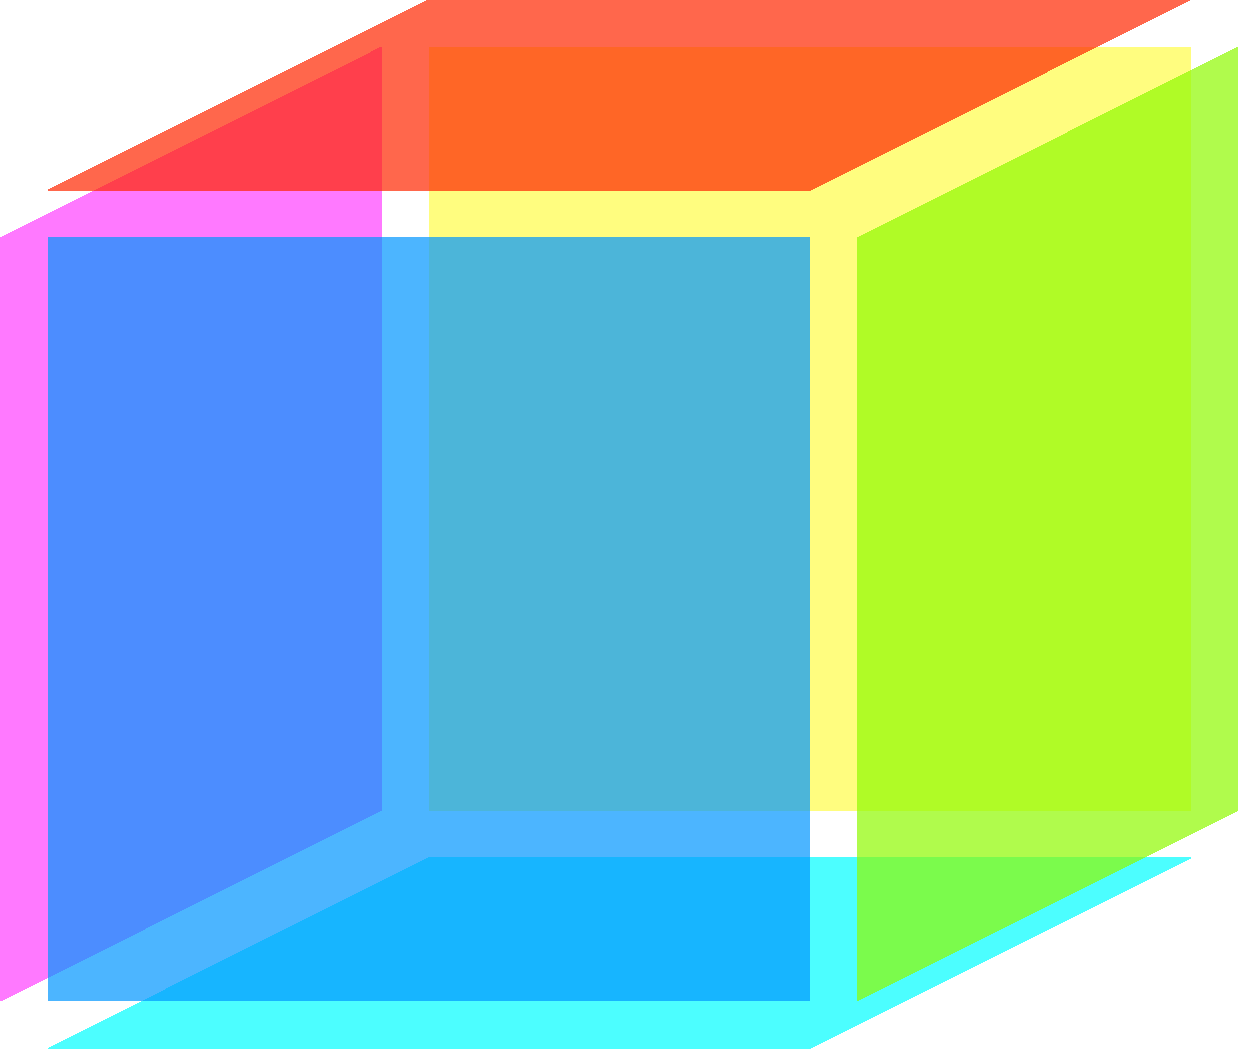
\includegraphics[width=\marginparwidth]{figs/brep}
\caption[Een kubus wordt gerepresenteerd als 6 vierkante 2D vlakken.]{In GIS wordt een kubus niet gerepresenteerd als een 3D volume maar als 6 vierkante 2D vlakken die tesamen de ruimte van de kubus omvatten.}
\label{fig:brep-sum-nl}
}
De resulterende representaties zijn efficiënt en relatief eenvoudig te gebruiken en veel methodes en applicaties zijn hierop gebaseerd.
Maar 2D representaties kennen hun beperkingen.
Problemen moeten worden versimpeld tot 2D;\ en het beheren van relaties tussen verschillende objecten is complex, vooral als deze relaties een tijdscomponent hebben of over verschillende detail-niveaus gaan.
Desalniettemin gaat veel GIS onderzoek over het verbeteren van de 2D representaties alsook het ontwikkelen van nieuwe methoden die op 2D representaties zijn gebaseerd.

Deze dissertatie bestudeerd een fundamenteel andere modelleer-benadering waarbij zowel ruimtelijke als niet-ruimtelijke kenmerken worden gemodelleerd als extra geometrische dimensies.
De kenmerken ``tijd'' en ``schaal'' worden daarbij specifiek bekeken (\reffignl{fig:axes-sum-nl}).
\marginpar{
\captionsetup{type=figure}
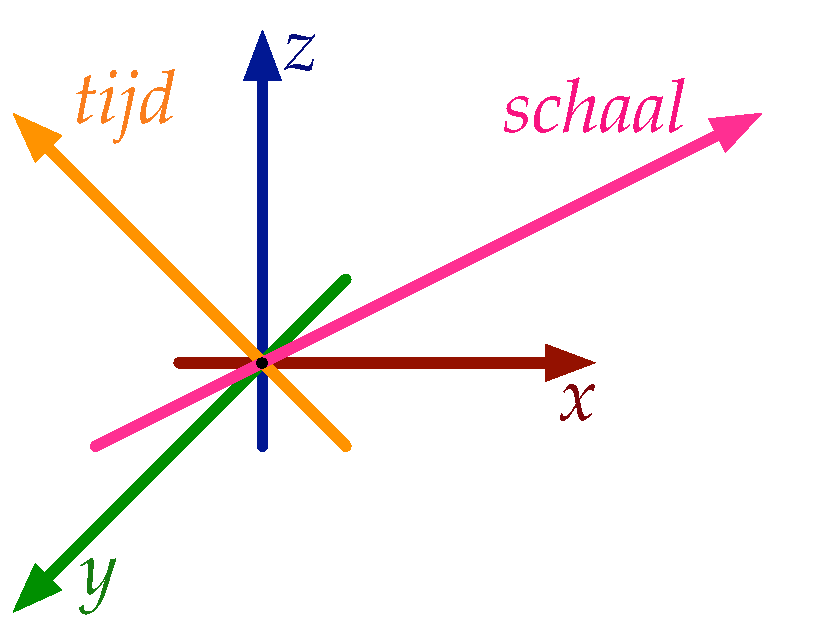
\includegraphics[width=\marginparwidth]{figs/axes-nl}
\caption{3D ruimte, tijd en schaal kunnen worden gemodelleerd als 5D ruimte.}
\label{fig:axes-sum-nl}
}
Eerdere onderzoeken naar het modelleren van tijd en schaal als extra dimensie zijn nooit verder gekomen dan een conceptuele beschrijving.
Dit onderzoek daarentegen beoogt de fundamentele aspecten van een multidimensionaal GIS te realiseren door hoger dimensionale ($n$D) representaties te ontwikkelen inclusief bewerkingsmethodes om deze $n$D geografische informatie te creëren, manipuleren en visualiseren.
\marginpar{
\captionsetup{type=figure}
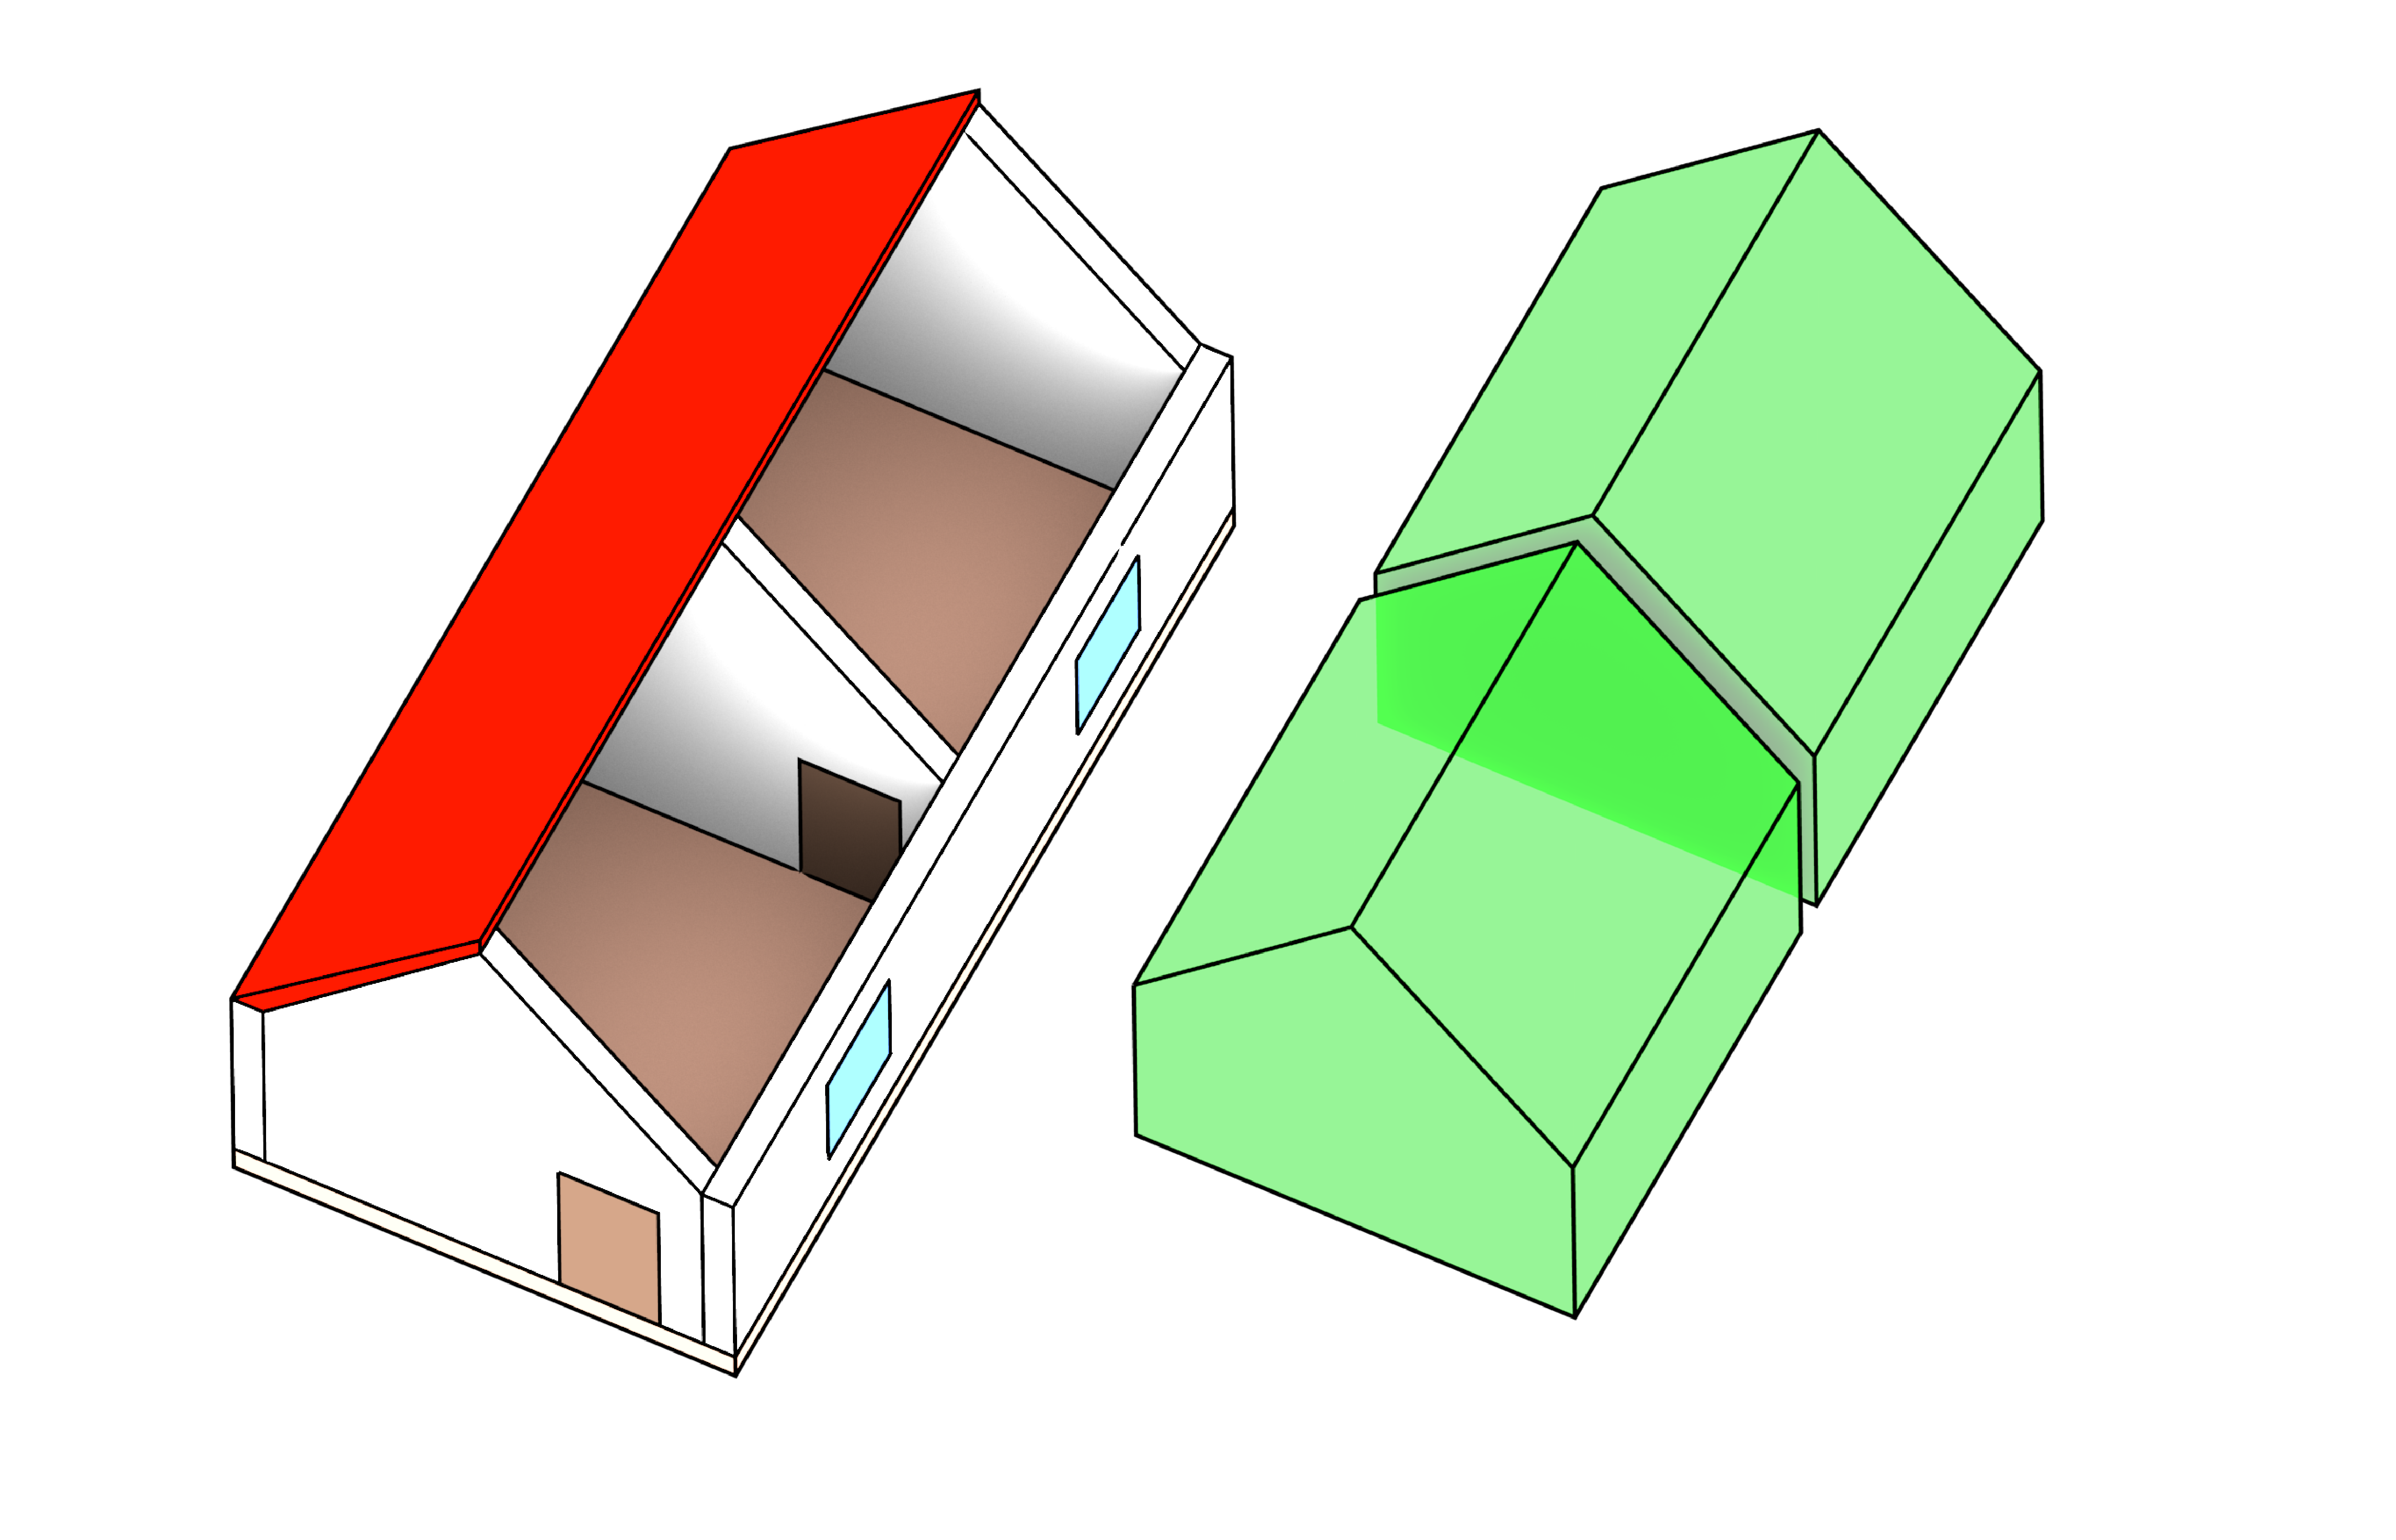
\includegraphics[width=\marginparwidth]{figs/space-filling}
\caption[3D ruimtelijke opdeling]{Een 3D ruimtelijke opdeling bestaat uit een set ruimte-vullende volumes zonder gaten en overlap.}
\label{fig:space-filling-sum-nl}
}
In deze thesis wordt aangetoond dat een $n$D benadering aan de ene kant veel computergeheugen vraagt om alle relaties over dimensies heen op te slaan.
Aan de andere kant is de aanpak zeer krachtig gebleken omdat een $n$D benadering op een doeltreffende en consistente manier geometrie met haar attributen opslaat.
Naast de objecten, kunnen ook alle topologische relaties tussen de objecten worden opgeslagen welke zich kunnen voordoen binnen en tussen iedere dimensie.
De in dit onderzoek voorgestelde aanpak is generiek en kan eenvoudig worden uitgebreid om andere niet-ruimtelijke aspecten te modelleren.
Hierdoor is data management waarbij de consistentie van geografische informatie wordt gegarandeerd over dimensies heen.
Bovendien kunnen hiermee krachtigere bewerkingen worden uitgevoerd zoals controleren of twee objecten op enig moment in de tijd aangrenzend zijn.

Om een $n$D ruimte te modelleren kan het best gestart worden met een $n$D ruimtelijke partitie (zonder gaten en overlap) (\reffignl{fig:space-filling-sum-nl}).
Conceptueel kan dit worden weergegeven als een $n$D \emph{simplicial complex} of een \emph{cell complex}.
Vervolgens kan dit worden geïmplementeerd via een \emph{simplex-based} datastructuur met een \emph{incidence graph}, bijvoorbeeld als een set van \emph{Nef polyhedra} of, zoals dat in dit onderzoek is gedaan, via geordende topologische modellen (\emph{cell-tuple} en \emph{generalised/combinatorial maps}).

Het construeren van computer representaties van $n$D objecten kan erg complex zijn.
Bestaande 2D/3D constructie methodes manipuleren \emph{combinatorial primitives} of maken gebruik van bewerkingen op primitieve-niveau (zoals Euler operatoren).
Deze gaan uit van onze intuïtie over 2D en 3D geometrieën en werken daarmee niet goed in hogere dimensies.
Hierdoor is het helaas heel makkelijk om invalide $n$D objecten te creëren die vervolgens moeilijk te bewerken zijn.
Dit probleem doet zich ook al voor in drie dimensies.

\marginpar{
\captionsetup{type=figure}
\subfloat[]{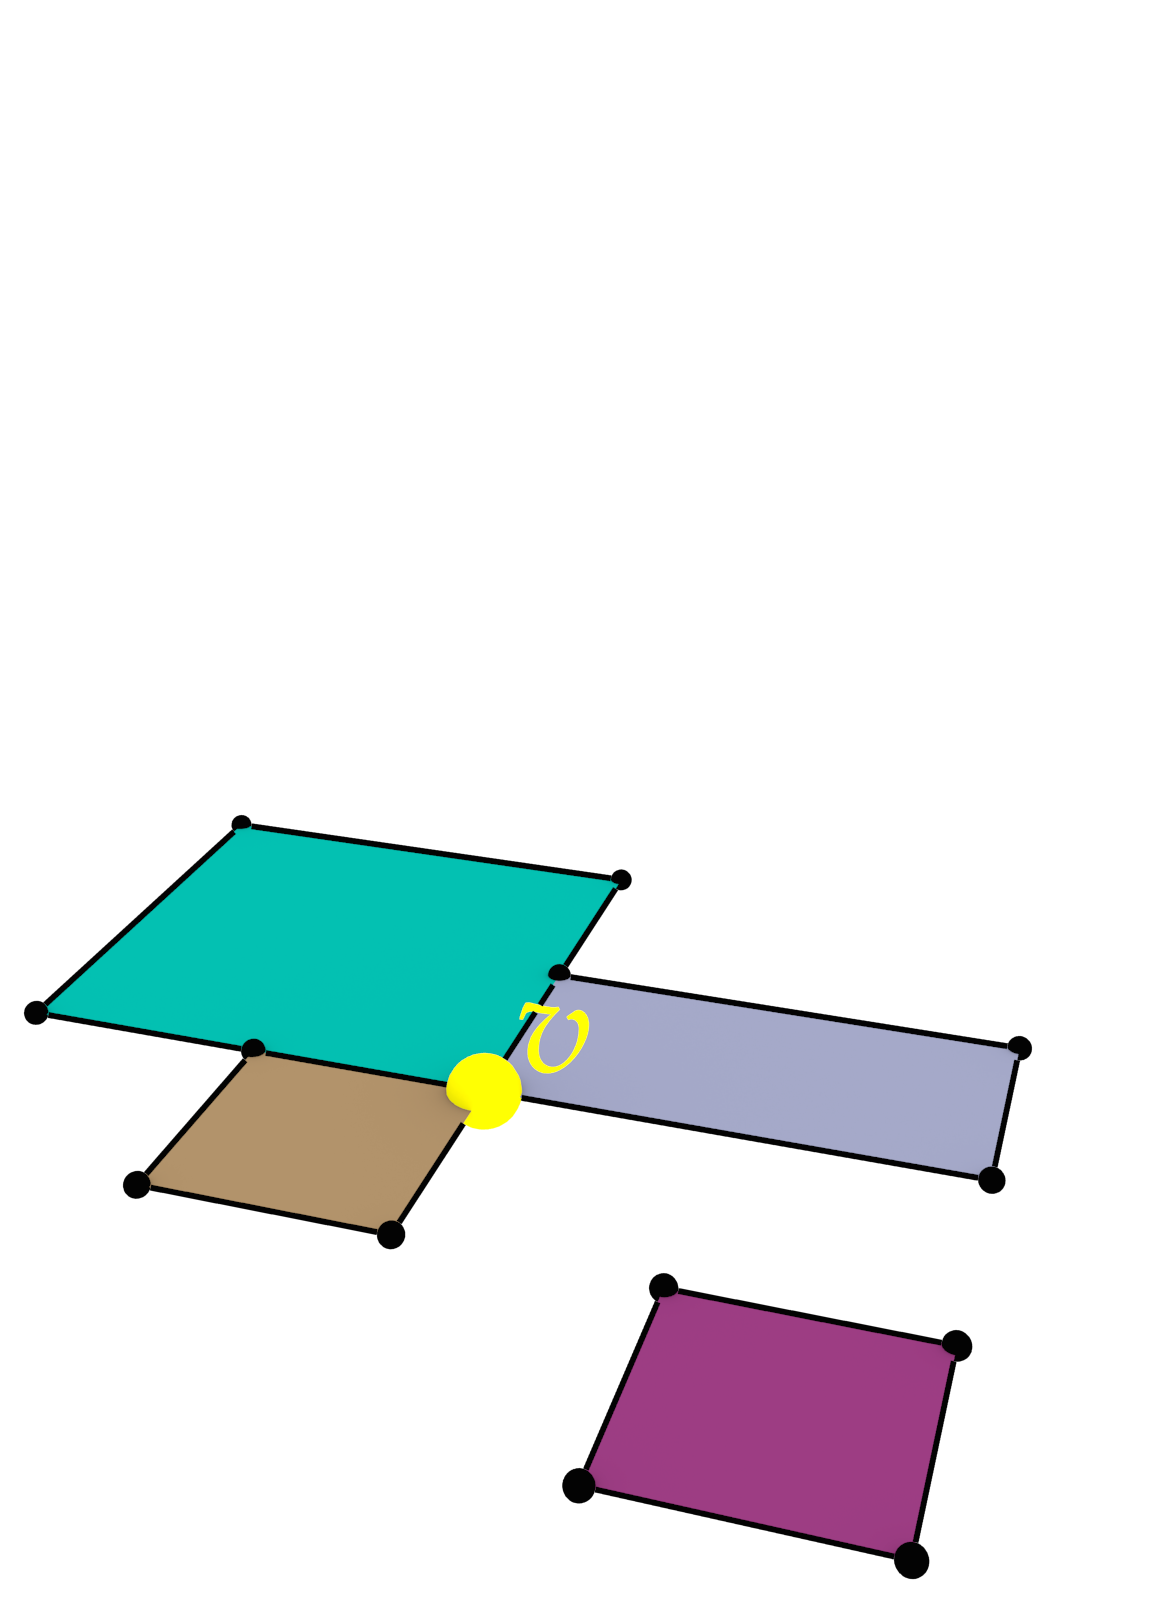
\includegraphics[width=\marginparwidth]{figs/extrusion-1}}\\
\subfloat[]{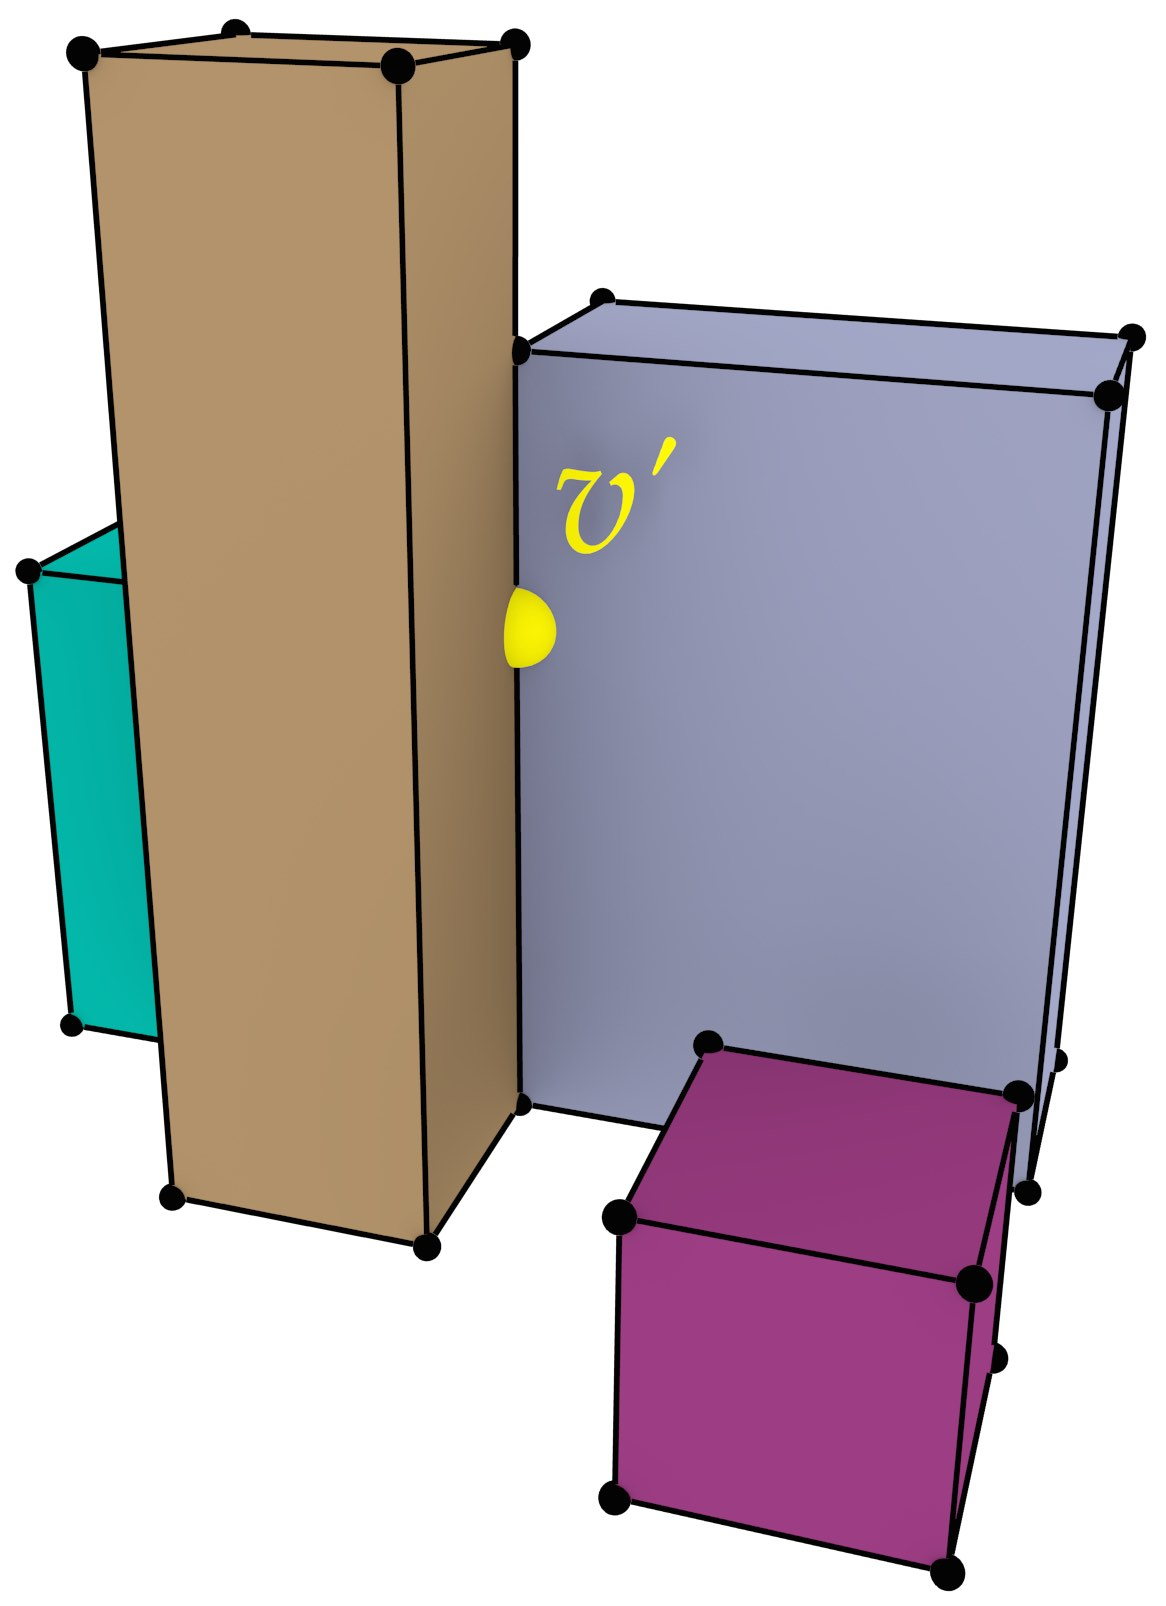
\includegraphics[width=\marginparwidth]{figs/extrusion-2}}
\caption[Een set polygonen wordt geconverteerd naar een set blokken.]{(a) een set polygonen wordt geconverteerd naar (b) een set blokken door de polygonen van 2D naar 3D op te trekken.}
\label{fig:extrusion-sum-nl}
}
\marginpar{
\captionsetup{type=figure}
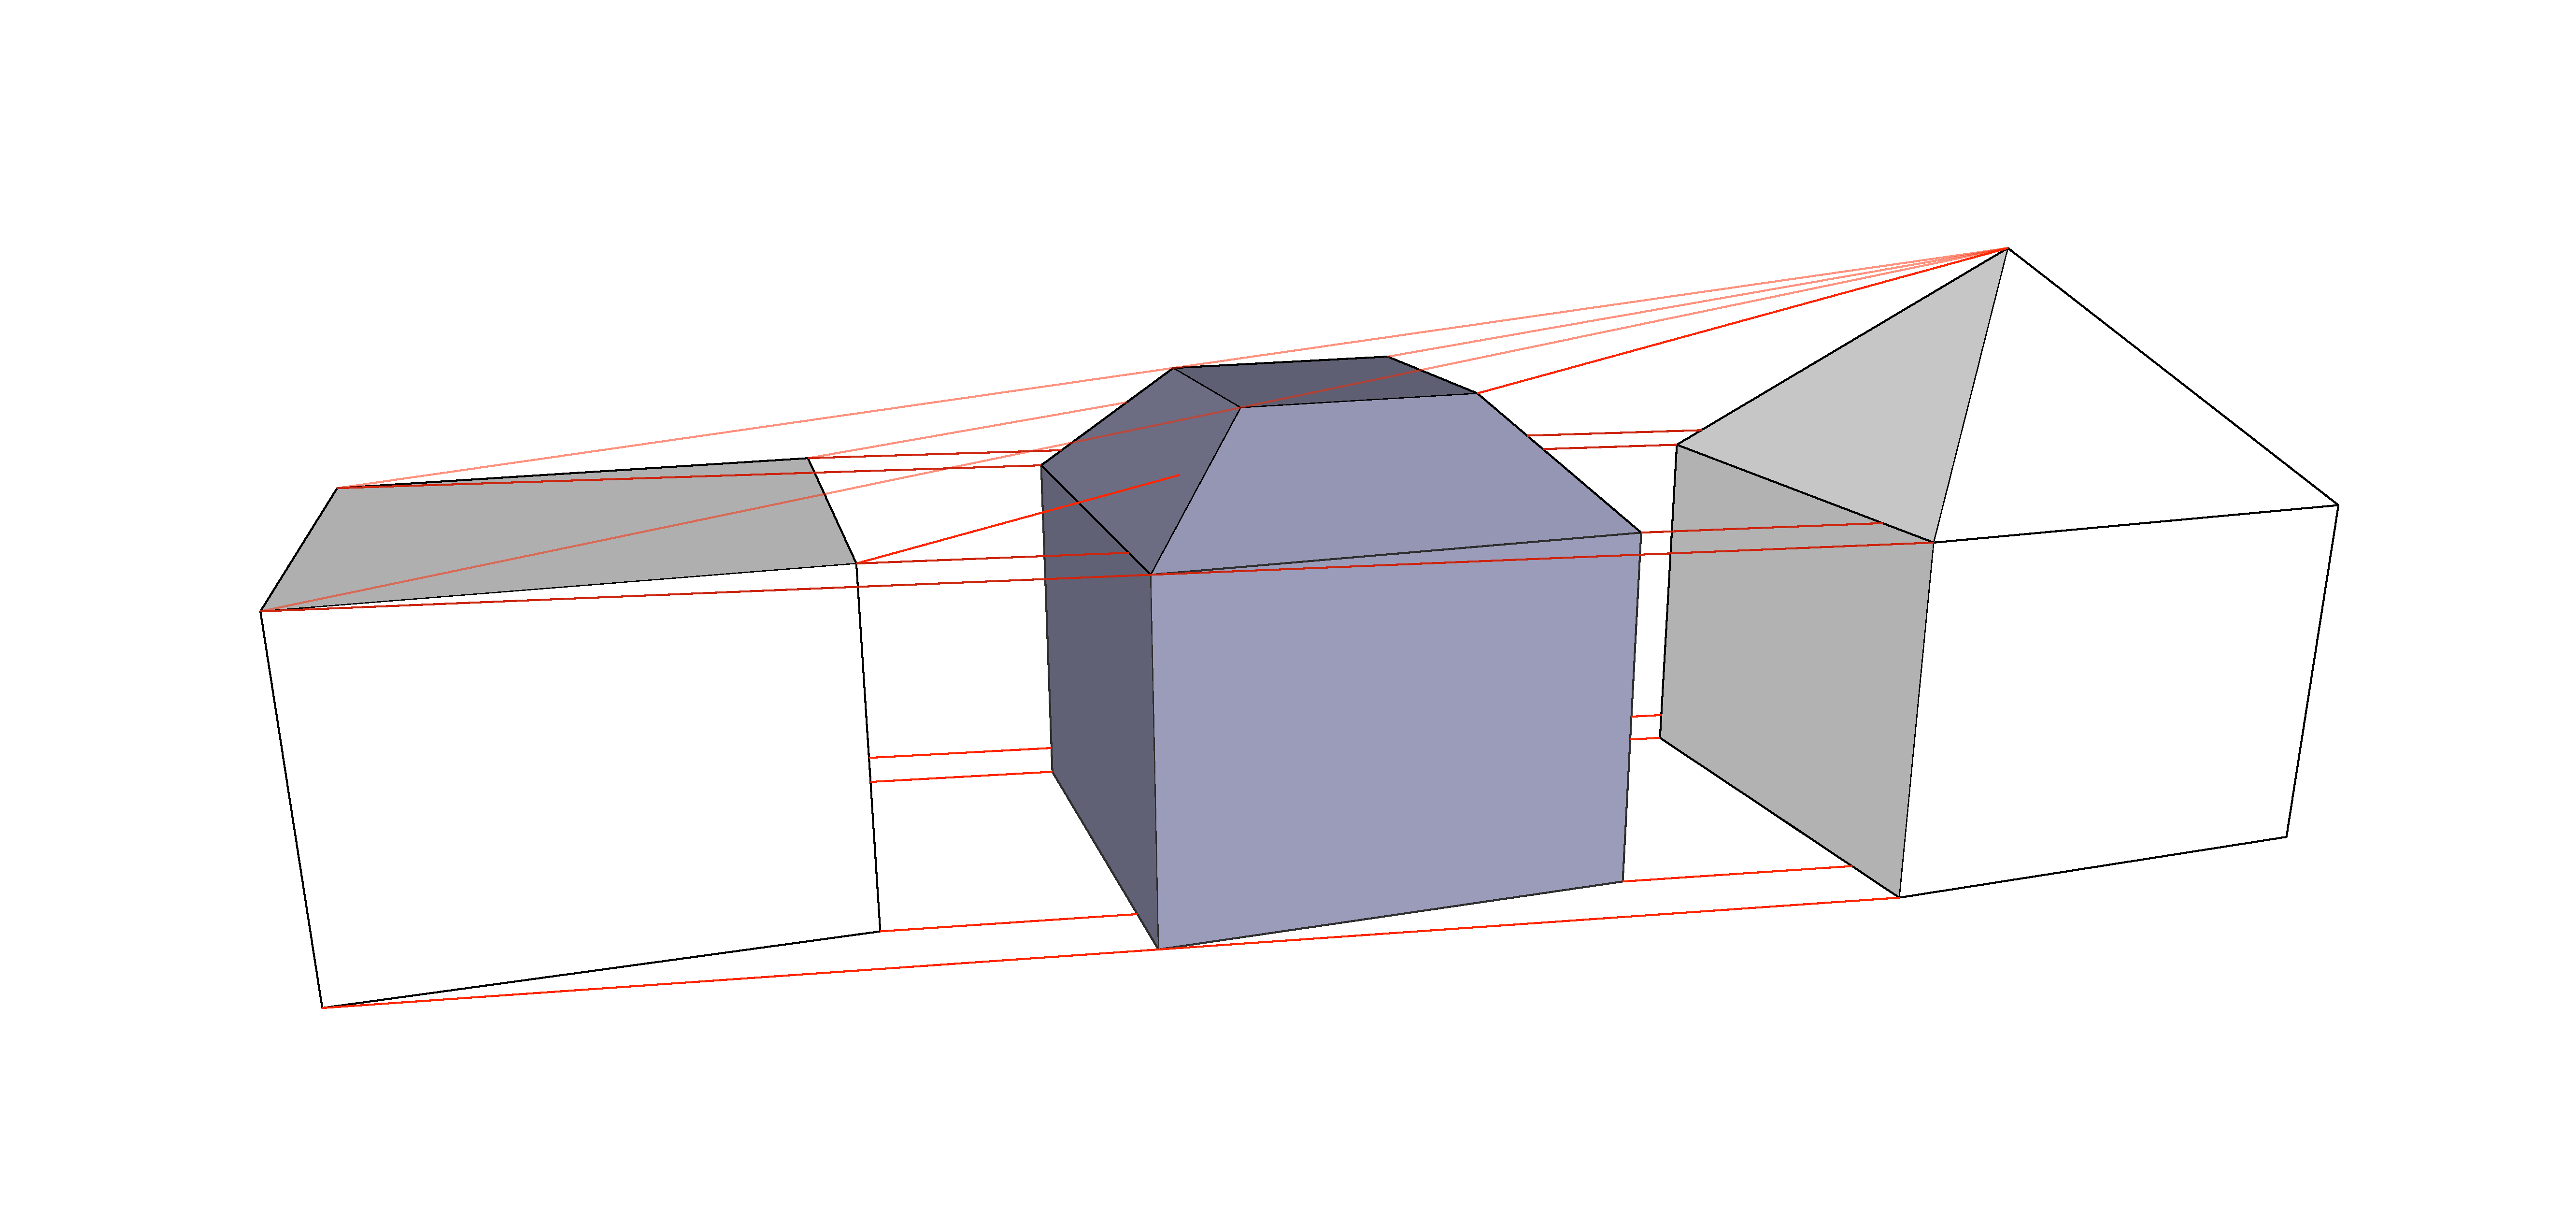
\includegraphics[width=\marginparwidth]{figs/link2}
\caption[Twee detailniveaus van een 3D model worden gelinkt tot een 4D model.]{Twee detailniveaus van een 3D model van een huis (links en rechts) worden gelinkt tot een 4D model.}
\label{fig:link-sum-nl}
}
In deze dissertatie is een manier onderzocht en ontwikkeld om eenvoudig valide representaties van $n$D objecten te construeren.
Daartoe zijn er drie methodes voorgesteld:
\emph{Extrusion} neemt een $(n-1)$D cell complex en een set van intervallen per cell en projecteert deze parallel aan een nieuwe as ten einde een $n$D cell complex te construeren (\reffignl{fig:extrusion-sum-nl}). 
\emph{Incremental construction} construeert een $n$D object op basis van zijn $(n-1)$-grens.
Via het \emph{linken} van verschillende representaties van hetzelfde 3D object op verschillende detailniveaus (LODs) met als resultaat een 4D model (\reffignl{fig:link-sum-nl}).

Om $n$D modellen te kunnen visualiseren en te kunnen bewerken in huidige software, is er een methode nodig om valide 2D/3D subsets af te leiden uit de $n$D data.
% Zo’n methode kent twee stappen: 1) het selecteren van een subset van de $n$D objecten uit het model en 2) de subset projecteren naar een lagere dimensie (2D of 3D).
Als opstap heeft dit onderzoek laten zien hoe een zowel orthografische als een perspectieve projectie van $n$D naar $(n-1)$D kan worden gedefinieerd.

Tenslotte heeft deze thesis alle hierboven genoemde concepten gevalideerd op $n$D data over de ``echte'' wereld.
Omdat er veel fouten voorkomen in deze data, zijn er in dit onderzoek ook methodes ontwikkeld om valide polygonen en een plenaire partitie te creëren op basis van \emph{constrained} triangulatie.
Daarnaast is er een methode ontwikkeld om polyhedra en ruimtelijke opdelingen te corrigeren door het ``snappen'' van primitieven op lagere dimensies en het verwijderen van overlap door middel van Boolean set bewerkingen op \emph{Nef polyhedra}.
Hierdoor zijn er testen gedaan met data tot 6D gebaseerd op ``echte'' GIS data, \emph{wat een goede basis is voor $n$D GIS}.\@

In de toekomst kan dit onderzoek worden uitgebreid met wijzigingsbewerkingen voor $n$D objecten, ``echte'' 4D ruimtelijk-temporele datasets en correctie methodes die de kwaliteit van de $n$D data garanderen.
Alle implementaties van deze dissertatie zijn publiekelijk beschikbaar via open source licenties.

}

\chapter{Resumen (Spanish summary)}

{\selectlanguage{spanish}

Nuestro mundo es tridimensional y complejo, cambiando continuamente a través del tiempo y mostrándose distinto a distintas escalas.
Aún así, cuando lo modelamos usando sistemas de información geográfica (SIG), generalmente usamos representaciones 2D, las cuales esencialmente consisten en conjuntos de puntos, líneas y polígonos enlazados entre sí (\reffiges{fig:brep-sum-es}).
\marginpar{
\captionsetup{type=figure}
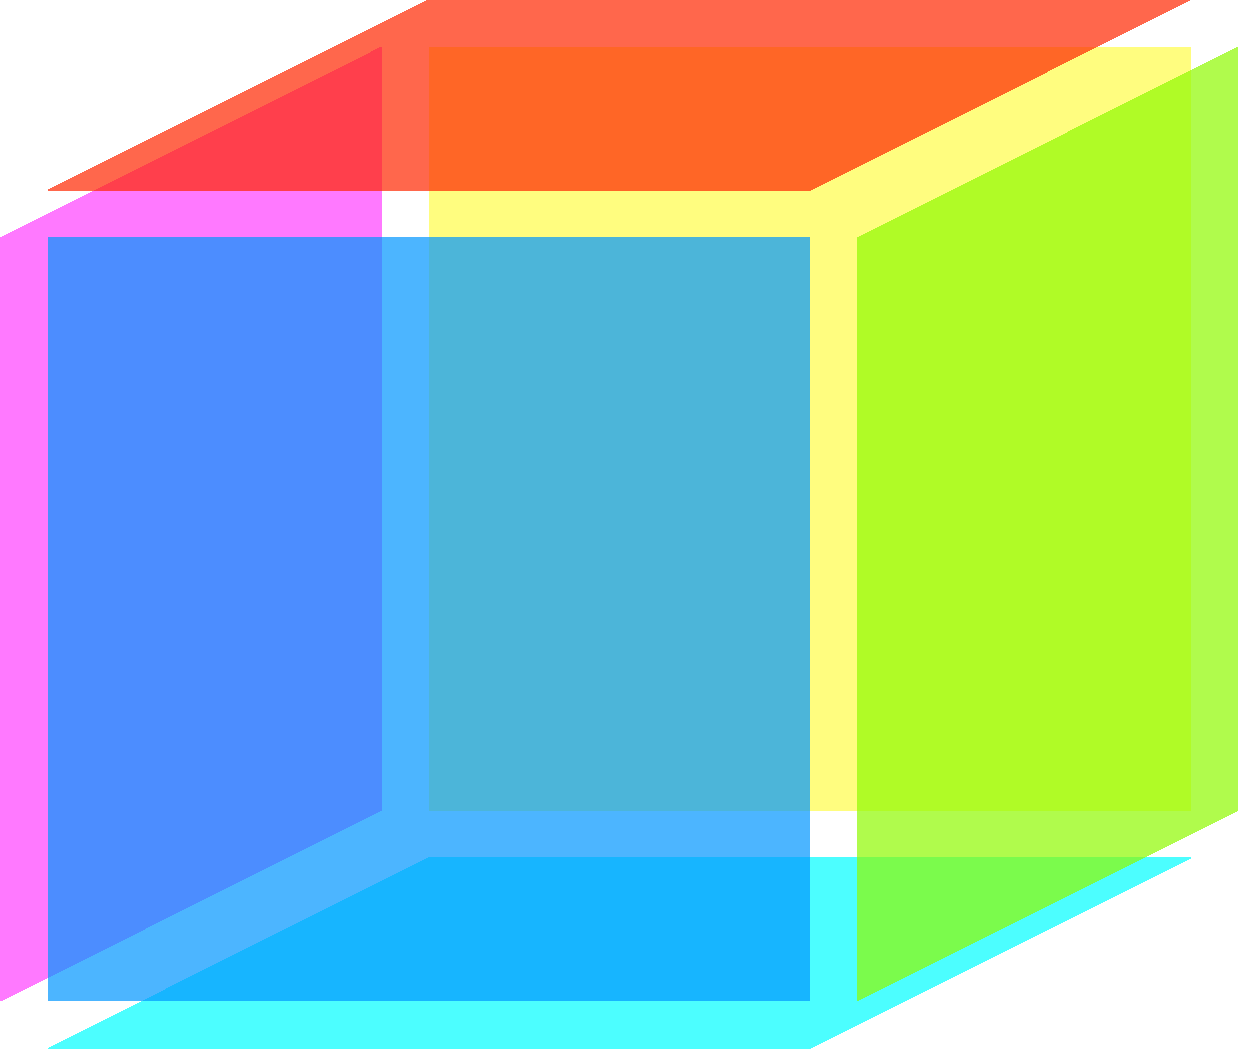
\includegraphics[width=\marginparwidth]{figs/brep}
\caption[Un cubo representado por las 6 caras cuadradas en su superficie]{En los SIG, un cubo no se representa como un sólido, sino como las 6 caras cuadradas en su superficie.}
\label{fig:brep-sum-es}
}
Estas representaciones son relativamente fáciles de usar y eficientes, y una gran variedad de métodos se han construido usándolas.
Sin embargo, las representaciones 2D son necesariamente restrictivas.
Nos fuerzan a reducir los problemas a dos dimensiones, limitan el tipo de objetos que podemos representar y dificultan guardar las relaciones entre diferentes objetos---especialmente cuando éstas son a través del tiempo y diferentes escalas.
A pesar de ello, la mayoría de la investigación en SIG se dedica a mejorar estas representaciones 2D, así como a desarrollar nuevos métodos que las usan para resolver problemas, sean éstos nuevos o antiguos.

Esta tesis explora un nuevo y fundamentalmente distinto paradigma de modelado---integrando características espaciales y espaciales como dimensiones en el sentido geométrico, específicamente apuntando hacia los casos del tiempo y la escala (\reffiges{fig:axes-sum-es}).
\marginpar{
\captionsetup{type=figure}
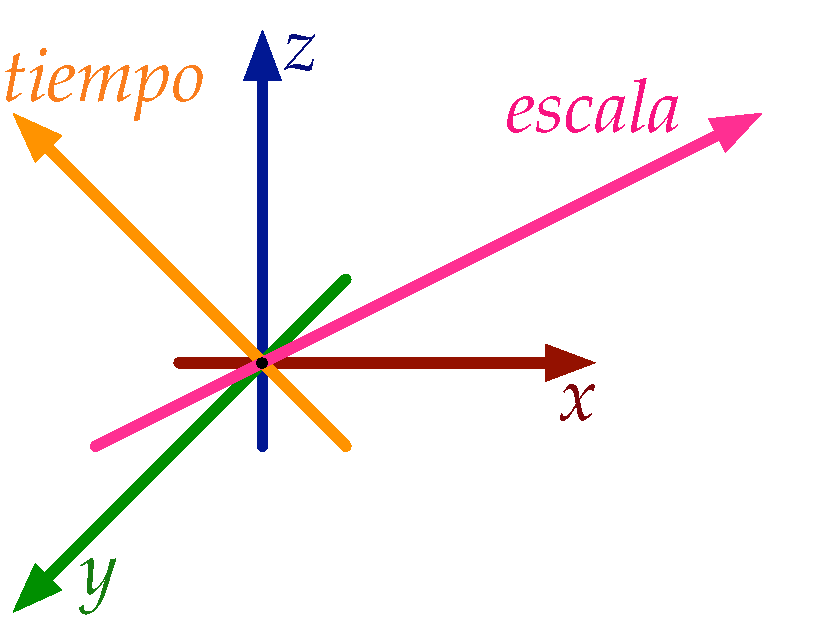
\includegraphics[width=\marginparwidth]{figs/axes-es}
\caption{El espacio 3D, el tiempo y la escala modelados como un espacio 5D.}
\label{fig:axes-sum-es}
}
A pesar de que este paradigma ha sido propuesto antes a un nivel conceptual, esta tesis tiene como objetivo llevarlo a cabo al \emph{implementar los aspectos fundamentales de un SIG de altas dimensiones}, desarrollando representaciones para objetos en altas dimensiones ($n$D), así como nuevos métodos que operen en ellas para crear, manipular y visualizar información geográfica.
Como esta tesis muestra, el paradigma de altas dimensiones tiene un alto consumo de memoria pero también es muy poderoso, proveyendo un método simple y consistente para guardar la geometría, los atributos y las relaciones topológicas entre objetos de cualquier dimensión.
Este paradigma genérico puede ser fácilmente extendido a otras características no espaciales, haciendo posible un mejor manejo de datos con consistencia a través de las dimensiones y operaciones más poderosas.
% , como verificar si dos objetos son adyacentes en algún momento.

Para poder modelar el espacio de altas dimensiones, es mejor considerar una partición espacial $n$D como una base (\reffiges{fig:space-filling-sum-es}), la que es conceptualizada como un complejo simplicial o celular.
\marginpar{
\captionsetup{type=figure}
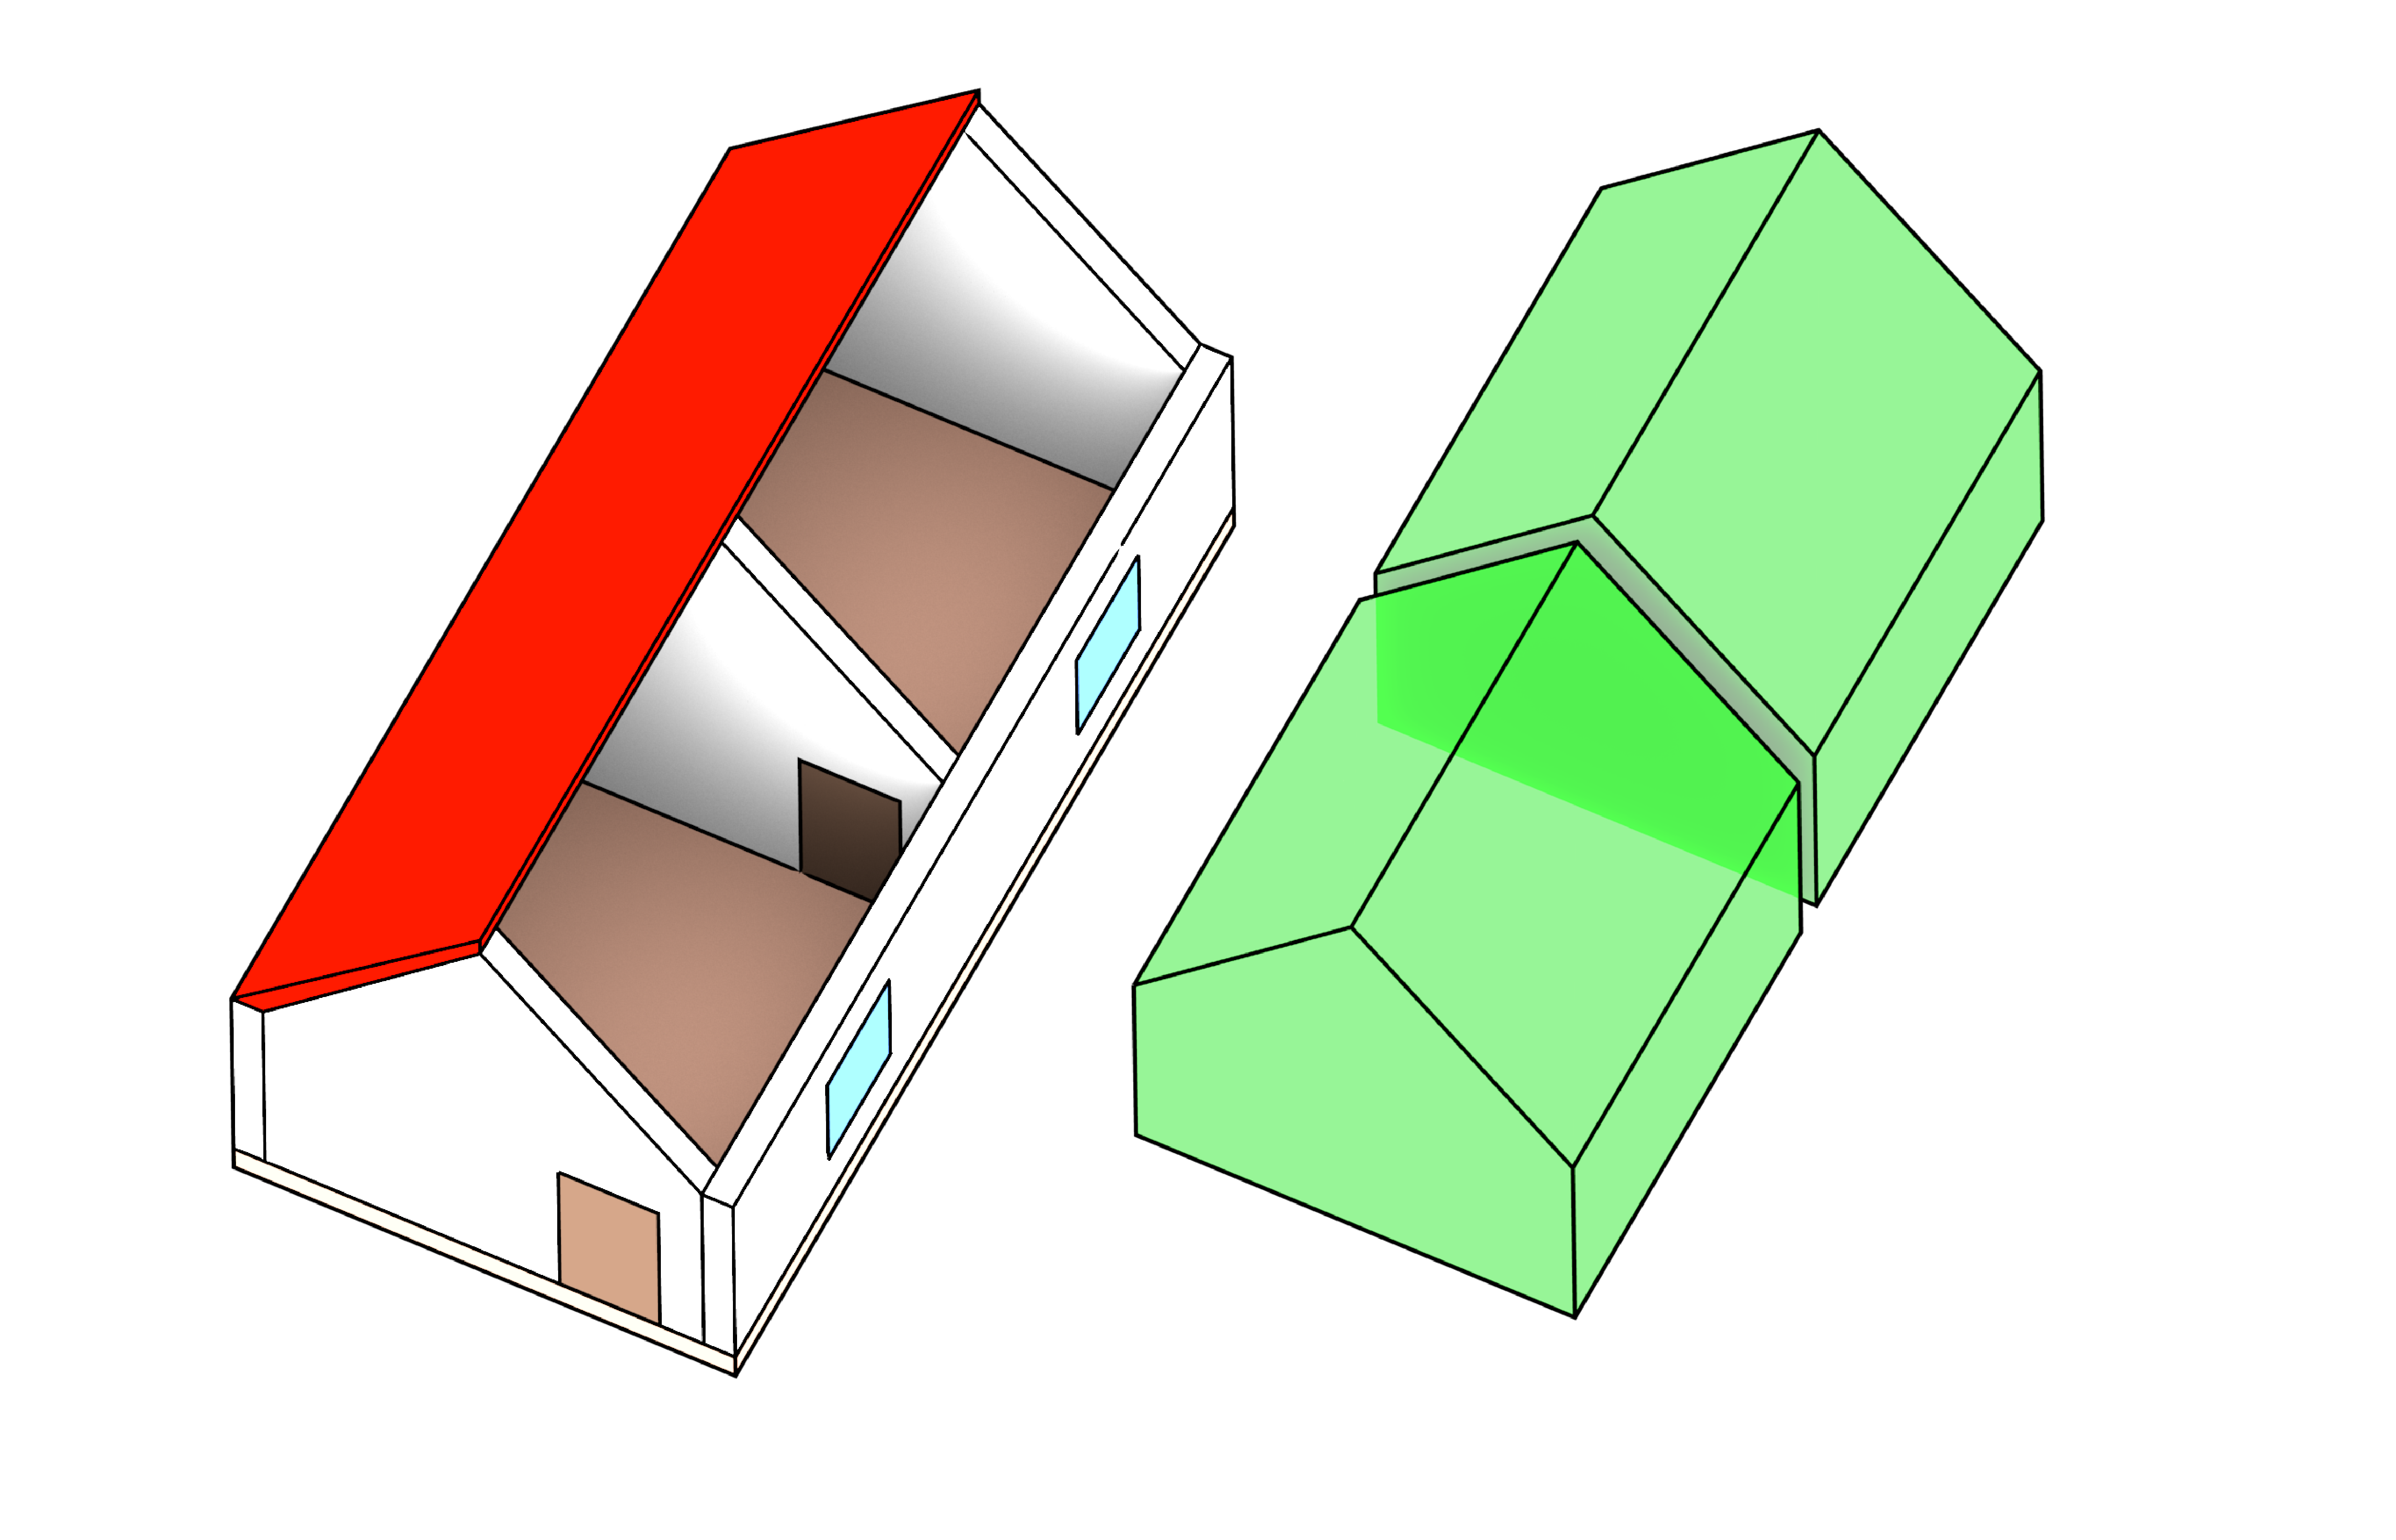
\includegraphics[width=\marginparwidth]{figs/space-filling}
\caption[Partición espacial 3D]{Una partición espacial 3D se compone de un conjunto de volúmenes que llenan el espacio sin huecos y sin solaparse entre ellos.}
\label{fig:space-filling-sum-es}
}
Éste puede entonces ser implementado con una estructura de datos basada en símplices, un grafo de incidencia, como un conjunto de poliedros Nef, o---como en esta tesis---usando modelos topológicos ordenados, como la tupla de células (\emph{cell-tuple}) o los mapas generalizados o combinatorios (\emph{generalised/combinatorial maps}).

\marginpar{
\captionsetup{type=figure}
\subfloat[]{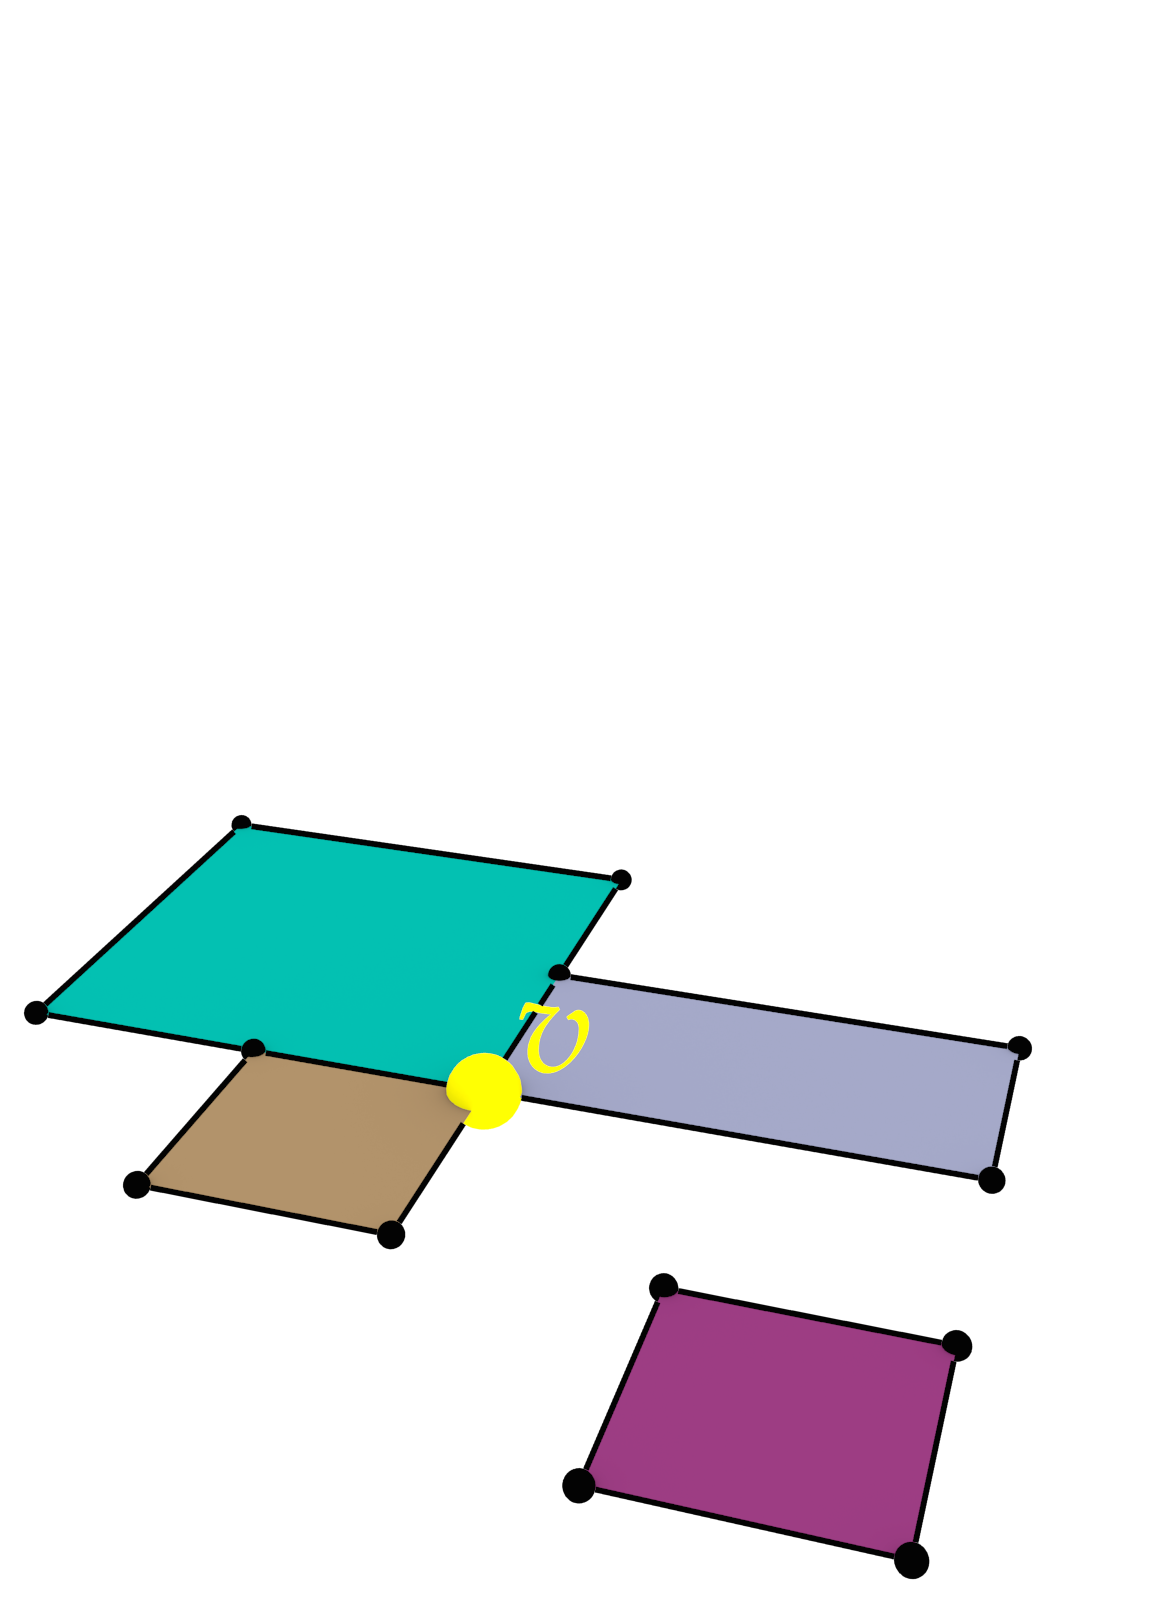
\includegraphics[width=\marginparwidth]{figs/extrusion-1}}\\
\subfloat[]{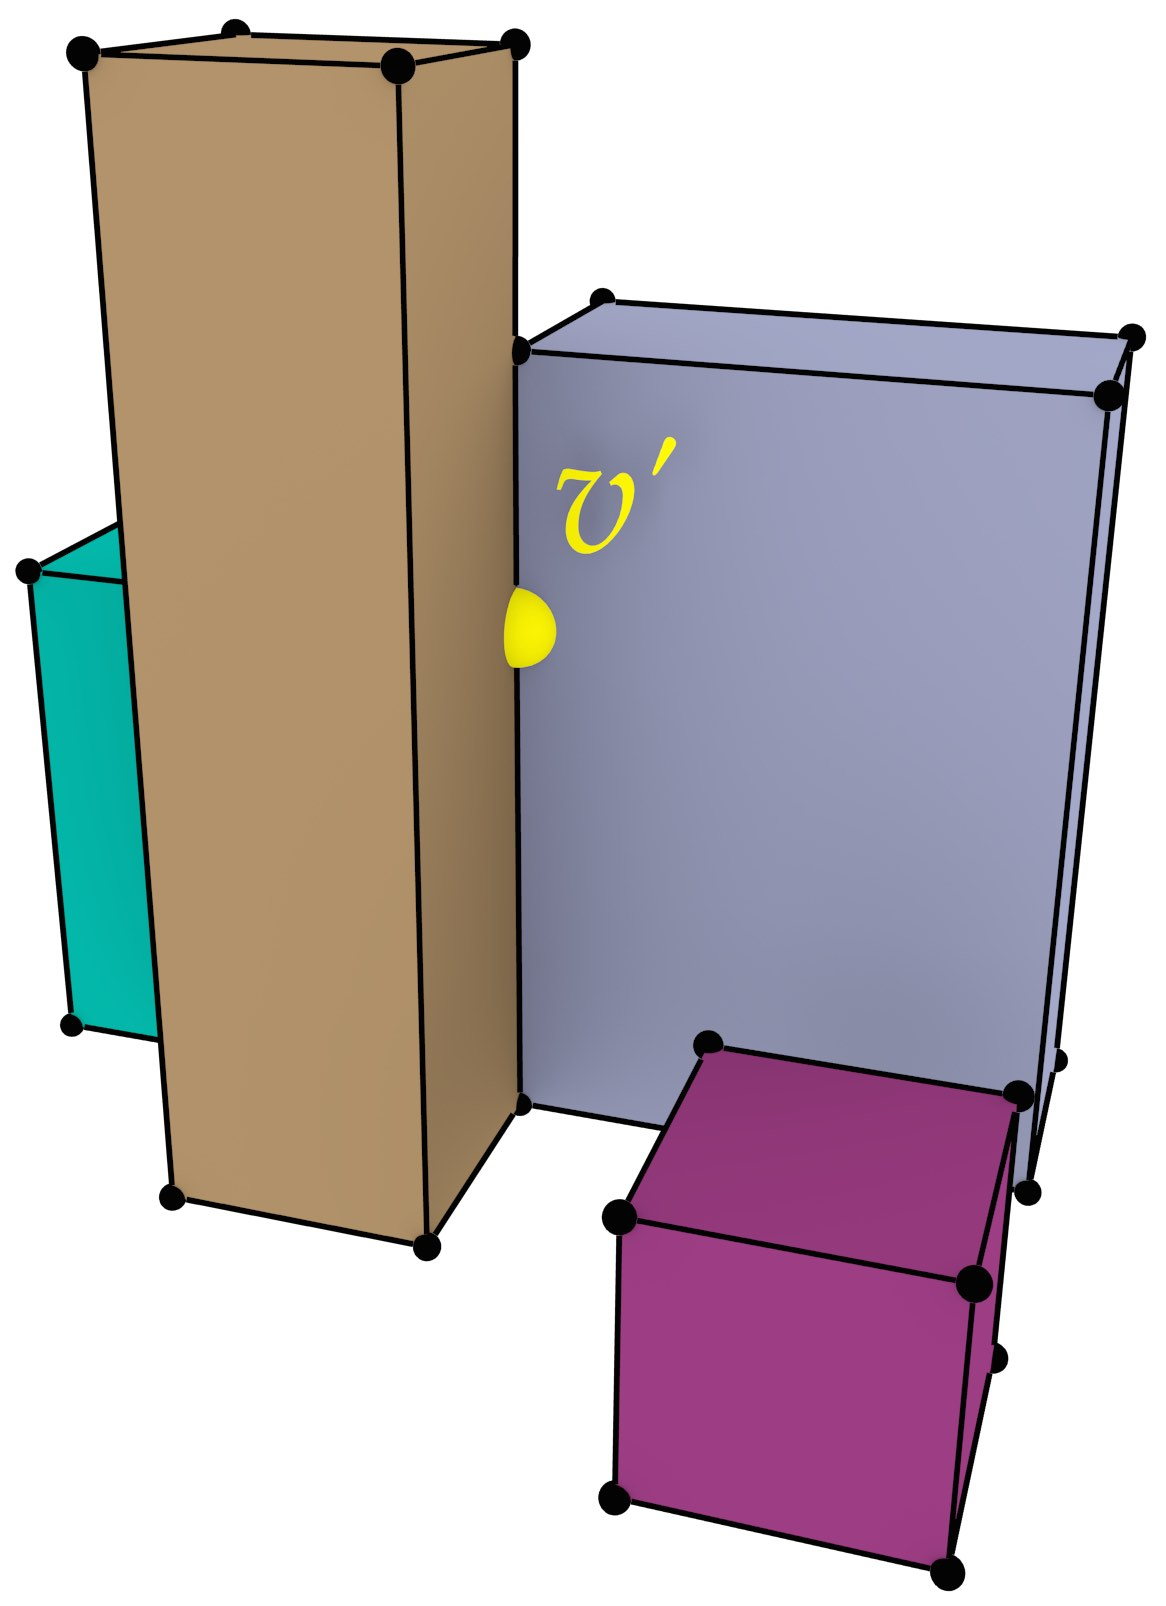
\includegraphics[width=\marginparwidth]{figs/extrusion-2}}
\caption[Un conjunto de polígonos se extrude en un conjunto de paralelepípedos.]{(a) Un conjunto de polígonos se convierte en (b) un conjunto de paralelepípedos al aplicar una extrusión 2D a 3D.}
\label{fig:extrusion-sum-es}
}
\marginpar{
\captionsetup{type=figure}
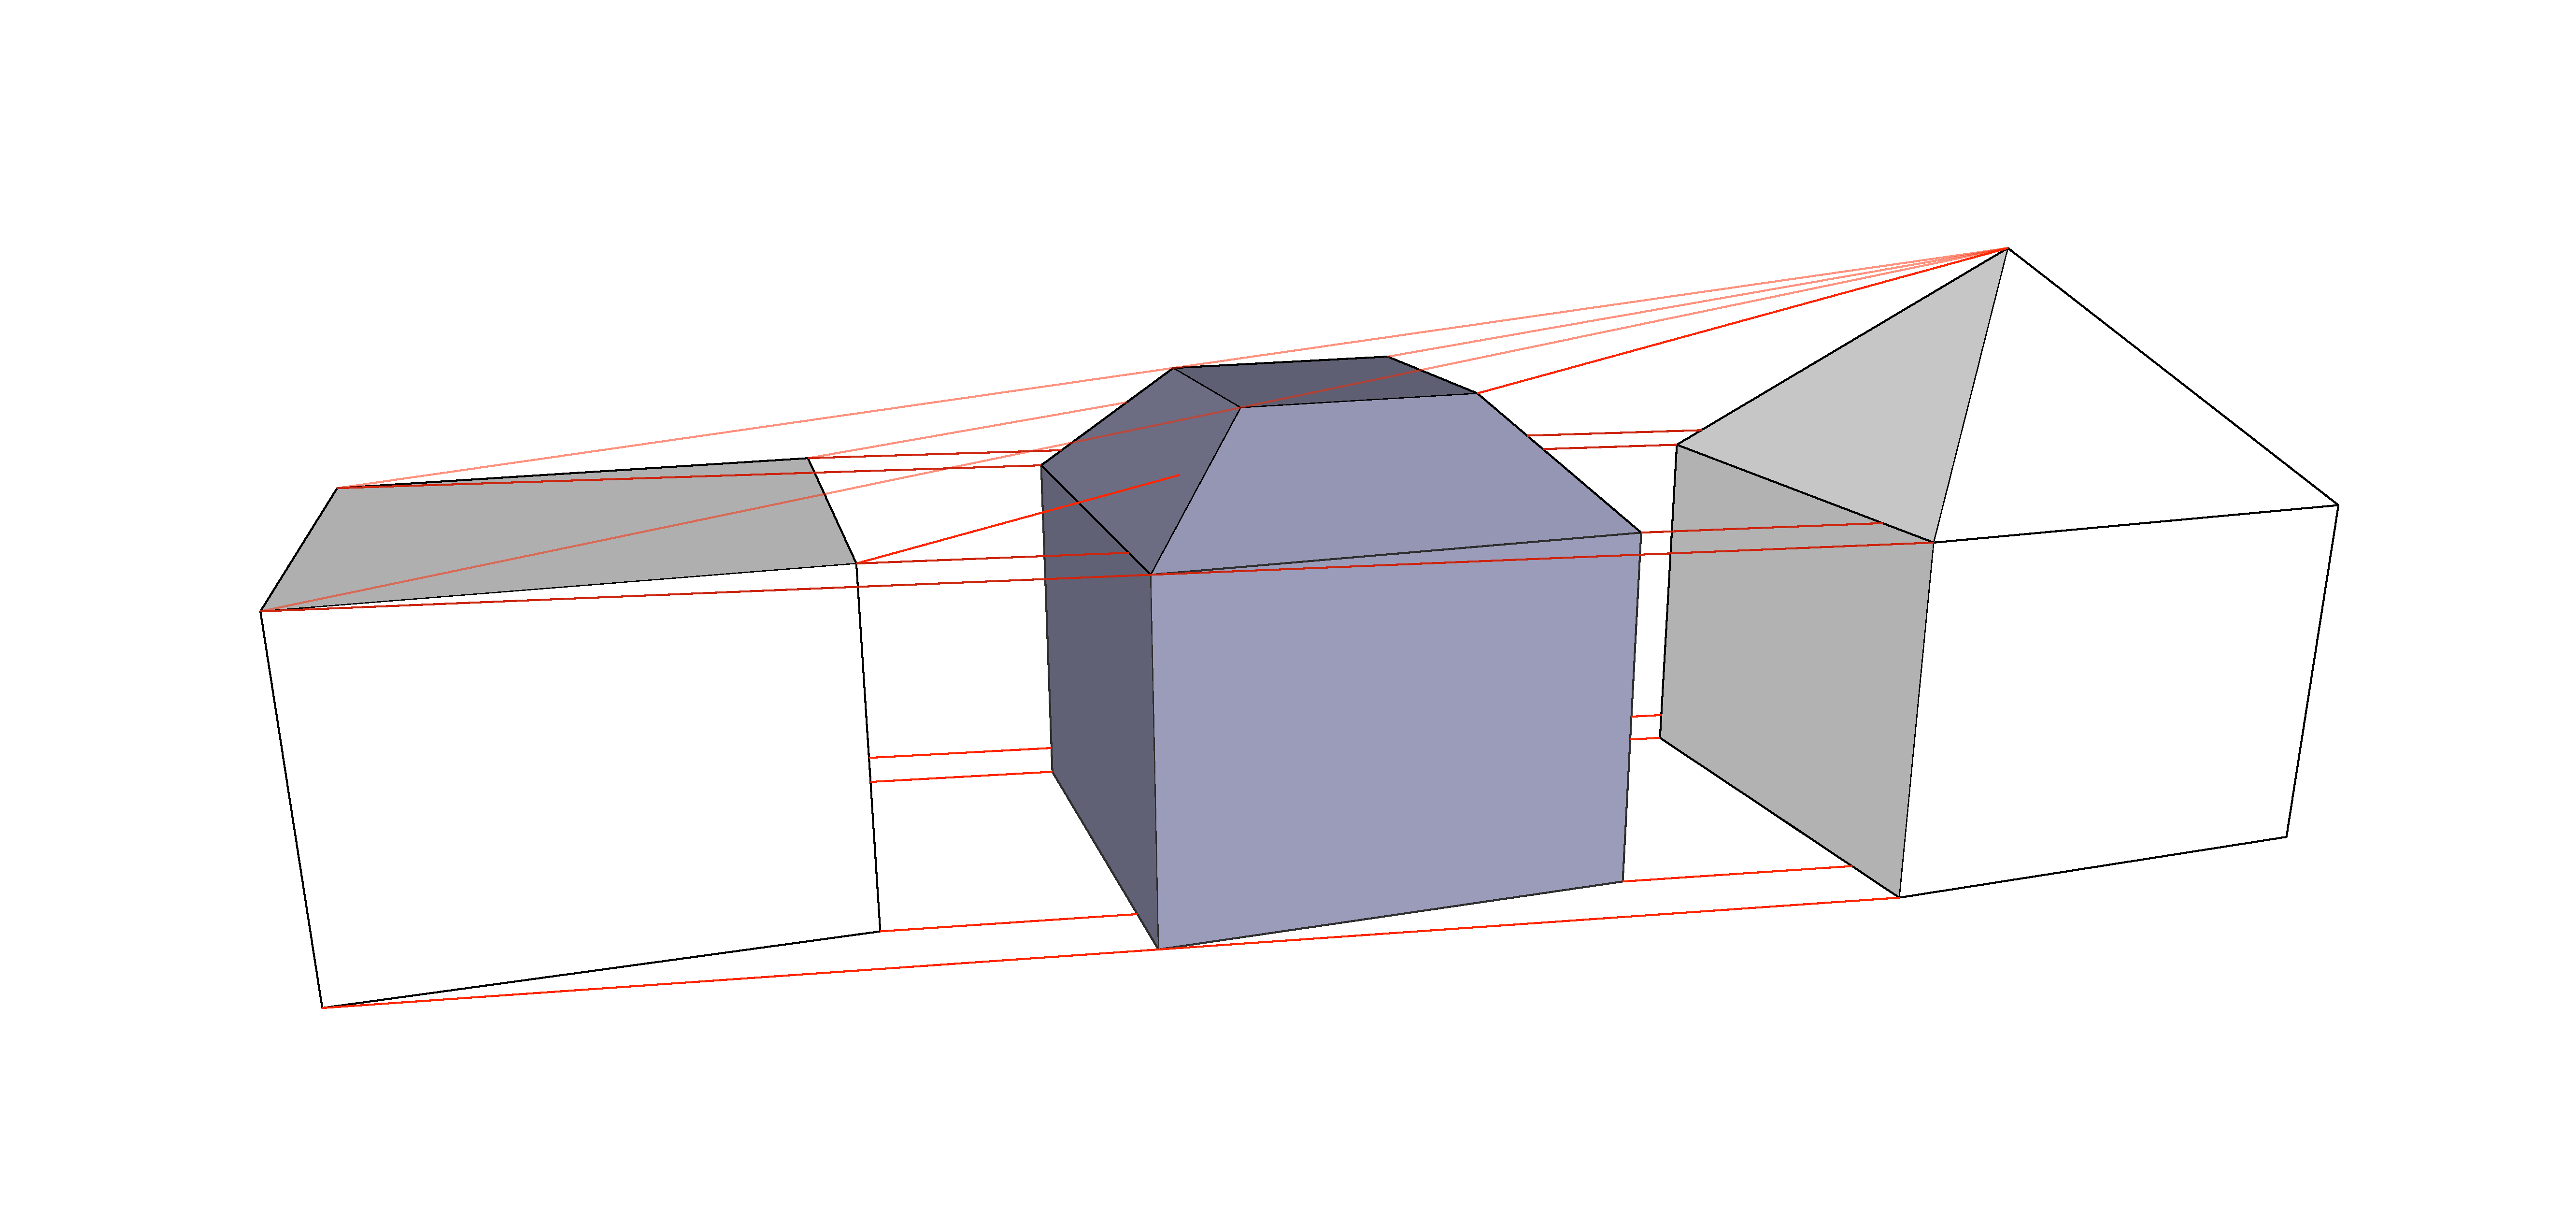
\includegraphics[width=\marginparwidth]{figs/link2}
\caption[Dos niveles de detalle de una casa se enlazan en un modelo 4D]{Dos niveles de detalle de una casa (izquierda y derecha) se enlazan en un modelo 4D.}
\label{fig:link-sum-es}
}
Crear representaciones de objetos en altas dimensiones puede ser complejo.
Los métodos comunes usados en 2D y 3D, como la manipulación directa de elementos combinatorios primitivos, o el uso de operaciones de construcción que operan al nivel de los elementos primitivos (como las operaciones de Euler), se basan en nuestra intuición de la geometría 2D/3D, y por lo mismo no funcionan bien en altas dimensiones.
Esto causa que sea demasiado fácil crear objetos inválidos, los cuales no pueden ser fácilmente interpretados o reparados---un problema que es extremadamente aparente incluso en tres dimensiones.

Esta tesis propone tres métodos novedosos para crear fácilmente representaciones de objetos en altas dimensiones, todos los cuales son intuitivos e intentar crear datos de salida válidos.
La \emph{extrusión} recibe un complejo celular $n-1$ dimensional y un conjunto de intervalos por cada célula, proyectándolos de forma paralela a un nuevo eje para crear un complejo celular $n$ dimensional (\reffiges{fig:extrusion-sum-es}).
La \emph{construcción incremental} describe un objeto $n$ dimensional basado en su frontera $n-1$ dimensional, desde la dimensión cero (puntos) y hacia arriba.
Finalmente, es posible construir un modelo 4D \emph{enlazando} una serie de modelos 3D a diferentes niveles de detalle (\reffiges{fig:link-sum-es}).

Para poder visualizar modelos en altas dimensiones, así como poder procesarlos en el software existente, es importante tener métodos para extraer de éstos subconjuntos significativos 2D/3D.
% Estos métodos consistirían de dos pasos: (i) seleccionar un subconjunto de los objetos en el modelo y (ii) proyectar este subconjunto a una dimensión menor.
Como un paso inicial hacia este tipo de métodos, esta tesis muestra como se pueden definir las proyecciones ortográficas y de perspectiva de $n$ dimensiones a $n-1$.

Finalmente, esta tesis tuvo un enfoque importante en validar los algoritmos con datos reales, lo cual sólo fue posible al desarrollar métodos para reparar datos inválidos, los cuales son comunes en la práctica.
Esta tesis por lo tanto contiene métodos para crear polígonos y particiones planares válidas usando una triangulación restringida de los datos de entrada, así como un método para reparar poliedros y particiones 3D juntando objetos (\emph{snapping}) de menores dimensiones y eliminando las partes que se solapan utilizando operaciones booleanas de conjuntos con poliedros Nef.
Esto permitió pruebas hasta en seis dimensiones basados en datos reales---\emph{una buena base para un SIG de altas dimensiones}.

En el futuro, el trabajo de esta tesis será extendido con operaciones de modificación en altas dimensiones, datos reales espaciales y temporales 4D, así como métodos de reparación de datos con garantías de calidad.
Todas las implementaciones hechas para esta tesis están disponibles públicamente bajo licencias de código abierto.

}
